% !TeX encoding = UTF-8
% !TEX TS-program = lualatex

% 山东第二医科大学入学与生活指南 © 2023-2024 by LinkChou is licensed under CC BY-SA 4.0. To view a copy of this license, visit https://creativecommons.org/licenses/by-sa/4.0 . Chinese version: https://creativecommons.org/licenses/by-sa/4.0/deed.zh-hans .

% 导入所需的package
\documentclass[a4paper,twoside,onecolumn,12pt,fontset=none]{ctexrep}%ctexreport文档类,fontset=none避免字体冲突警告
%\usepackage{fontspec}%在使用Overleaf编译时取消此行以使字体设置生效,详见ReadMe文件结尾的说明
\usepackage{bxtexlogo}%LaTeX logo(禁止换用hvlogos,因其会重定义部分字体导致报错)
\usepackage{fancyhdr,titlesec}%标题、脚注格式
\usepackage{ulem,xcolor}%段落、文字格式
\usepackage{graphicx}%插入图片
\usepackage{float}%图表位置,如表格过长致横向排版已不可能,应加用adjustboxs宏包排版旋转表格
\usepackage{tabularray}%表格排版
\usepackage{enumitem}%列表排版
\usepackage[a4paper, hmargin=1.5cm, top=1.5cm, bottom=2cm, headheight=0pt, ignorehead]{geometry}%页边距与排版
\usepackage[bookmarksnumbered=true, hidelinks, allbordercolors={0 0 0}, pdfborderstyle={/S/U/W 1}]{hyperref}%超链接
\usepackage{texosquery}%获取秒数及时间
\usepackage{datetime2}%扉页基本时间及格式
%\usepackage{showframe}%显示页面布局与边框,仅Preview版本排查错误

% 设置文档标题
\hypersetup{pdftitle={山东第二医科大学指南 SDSMU-Companion}}

% 重设定标题与正文间距
\ctexset{
    chapter={
        beforeskip=0ex,
        afterskip=4ex
    },
    section={
        beforeskip=0ex,
        afterskip=0ex
    },
    subsection={
        beforeskip=0ex,
        afterskip=0ex
    },
    subsubsection={
        beforeskip=0ex,
        afterskip=0ex
    }
}

% 重定义部分logo符号以免冲突
\bxtexlogoimport{LuaLaTeX}
\bxtexlogoimport{XeLaTeX}
\bxtexlogoimport{LaTeXe}

% 重定义文章字体为梦源宋体(不使用思源宋体的原因是思源的行高过高)
\setmainfont[BoldFont=Dream Han Serif CN W20.ttf]{Dream Han Serif CN W7.ttf}
\setCJKmainfont{Dream Han Serif CN W7.ttf}[BoldFont=Dream Han Serif CN W20.ttf]
\setCJKsansfont[BoldFont=Dream Han Serif CN W20.ttf]{Dream Han Serif CN W7.ttf}

% 段间距与行间距重设定
\setlength{\parskip}{.75ex plus 5pt minus 8pt}
\setlength{\lineskip}{.5ex plus 5pt minus 8pt}

% 页眉页脚
\pagestyle{fancy}
\fancyhf{}
\fancyfoot[C]{\thepage}

% 脚注格式(无分割线)
\renewcommand{\headrulewidth}{0pt}
\renewcommand{\footrulewidth}{0pt}
\renewcommand{\thefootnote}{\fnsymbol{footnote}}

% 列表样式重定义
\setlist[enumerate,1]{label=\arabic*.}
\setlist[enumerate,2]{label=(\arabic*)}
\setlist[enumerate,3]{label=[\arabic*]}
\setlist[enumerate,4]{label=<\arabic*>}
\setlist[enumerate]{itemsep=0pt}

%重定义表格脚注字体大小并增加“no-caption”表格样式
\DefTblrTemplate{note-text}{default}{{\footnotesize\InsertTblrNoteText}}
\DefTblrTemplate{remark-tag}{default}{{\footnotesize\bfseries\InsertTblrRemarkTag}}
\DefTblrTemplate{remark-text}{default}{{\footnotesize\InsertTblrRemarkText}}
\NewTblrTheme{no-caption}{
    \SetTblrTemplate{caption}{empty}
}

%重定义表格换页时内容
\DefTblrTemplate{contfoot-text}{default}{续下页}
\DefTblrTemplate{conthead-text}{default}{(续)}

% 设置校徽命令
\newcommand{\BackgroundPic}{
    \noindent\parbox{\paperwidth}{
        \centering
        \vspace*{400pt}
        
\includegraphics[width=5cm]{resources/sundry/logo.pdf}
    }
}

% 颜色重设定
\newcommand{\colored}[4]{
    \textcolor[RGB]{#1,#2,#3}{#4}
}

% 时间样式重设定
\newcommand{\CurrentCustomTime}{
    \DTMsavenow{Compiled_time}%保存编译时间
    \DTMfetchyear{Compiled_time}.%
    \DTMtwodigits{\DTMfetchmonth{Compiled_time}}.%
    \DTMtwodigits{\DTMfetchday{Compiled_time}}\quad%
    \DTMtwodigits{\DTMfetchhour{Compiled_time}}:%
    \DTMtwodigits{\DTMfetchminute{Compiled_time}}:%
    \DTMtwodigits{\DTMfetchsecond{Compiled_time}}\quad%
    GMT\DTMfetchTZhour{Compiled_time}:\DTMfetchTZminute{Compiled_time}
}

\begin{document}

% 扉页

% 添加标题校徽背景图
\AddToHookNext{shipout/background}{\BackgroundPic}

% 题目
\title{%
\normalsize
\vspace{100pt}
{\Huge\textbf{山东第二医科大学指南}}\\[10pt]
(简称:\colored{171}{79}{36}{321指南})\\[30pt]
%{\large\textbf{\colored{59}{100}{220}{3.0.7}}}\vspace*{-25pt}}
{\large\colored{255}{0}{0}{320-Preview}}\vspace*{-25pt}}
\author{LinkChou\thanks{Compiled by \LaTeXe, CC BY-SA 4.0 LICENSE.\qquad%
        \uline{\href{Mailto:LinkChou@yandex.com}{Mailto: LinkChou@yandex.com}}\\
        \textbf{敬告:}\\
        \indent\indent 力薄才疏,不免舛误,敬请绳愆纠缪。具体内容均以学校官方为准,如有变更恕不另行通知。}
    \and 山东第二医科大学频道}
\date{\colored{36}{98}{105}{\CurrentCustomTime}}
\maketitle

% 脚注样式重设定
\renewcommand{\thefootnote}{\arabic{footnote}}

\tableofcontents%标题、目录

% 特别感谢(尤其感谢我自己)
\chapter*{特别感谢}
%使用表格排版感谢
\vspace*{-4ex}
\begin{tblr}[
        long,
        theme=no-caption
    ]{
        cells={c,m},
        row{1,3,5,7,9} = {5ex},
    }
    {\large\textbf{审核校对}}                                                             \\
    {周大为}                                                                              \\
    {\large\textbf{内容改进}}                                                             \\
    {
    \uline{\href{https://xchb.sdsmu.edu.cn}{山东第二医科大学临床医学院}}                 \\
    \uline{\href{https://xchb.sdsmu.edu.cn}{山东第二医科大学党委宣传部}}                 \\
    \uline{\href{https://pd.qq.com/s/7mekdr5ve}{山东第二医科大学频道}}
    }                                                                                     \\
    {\large\textbf{项目结构与内容}}                                                       \\
    {
    \uline{\href{https://zjuers.com/welcome}{浙江大学本科新生指引}}                      \\
    \uline{\href{https://survivesjtu.gitbook.io/survivesjtumanual}{上海交通大学生存手册}} \\
    \uline{\href{https://sustech-application.com}{南方科技大学飞跃手册}}                 \\
    \uline{\href{https://survivesjtu.github.io/SJTU-Application}{上海交通大学飞跃手册}}  \\
    \uline{\href{https://gitee.com/hanyaner/witjij}{武工大计院新生入学建议}}
    }                                                                                     \\
    {\large\textbf{格式与疑难问题}}                                                       \\
    {
    {\uline{\href{https://github.com/CTeX-org/forum/issues}{GitHub CTeX Forum}}、%
            \uline{\href{https://tex.stackexchange.com}{TeX StackExchange}}、%
    \uline{\href{https://www.latexstudio.net}{LaTeX工作室}}}                             \\
    {\uline{\href{https://liam.page}{始终(Liam Huang)}}、%   
    \uline{\href{https://ctan.org/pkg/latexindent}{latexindent.pl}}}            \\
    {\uline{\href{https://github.com/lvjr/tabularray}{tabularray}}、%
    \uline{\href{https://gitee.com/nwafu_nan/tabularray-doc-zh-cn}{tabularray-doc-zh-cn}}}
    }                                                                                     \\
    \\
    {\large\textbf{\textcolor{red}{其他所有为本指南、地图提供建议与改进意见的同学、教师等}}}
\end{tblr}

\begin{tblr}[
        long,
        theme=no-caption
    ]{
        cells={c,m},
        cell{3}{1} = {c=3}{},
        column{2} = {2em},
    }
    {\large\colored{22}{120}{255}{\textbf{支付宝}}}           &  & %
    {\large\colored{5}{192}{95}{\textbf{微信}}}                    \\
    
\includegraphics[height=4cm]{resources/pay/Ali_pay.png}   &  & %
    
\includegraphics[height=4cm]{resources/pay/Wechat_pay.png}     \\
    \colored{255}{20}{147}{感觉有帮助?请我喝杯咖啡(〃∀〃)} &  &
\end{tblr}
%特别感谢
% 前言
\chapter[指南简介]{指南简介}

\section[许可证及项目信息]{许可证及项目信息}
山东第二医科大学指南 © 2023-2024 by \textcolor{blue}{$LinkChou$} is licensed under CC BY-SA 4.0. To view a copy of this license, visit \uhref{http://creativecommons.org/licenses/by-sa/4.0}{http://creativecommons.org/licenses/by-sa/4.0}.

Gitee仓库地址:\uhref{https://gitee.com/LinkChou/sdsmu_welcome_tex}{https://gitee.com/LinkChou/sdsmu\_welcome\_tex}

Github仓库地址:\uhref{https://github.com/Mikachu2333/sdsmu_welcome_tex}{https://github.com/Mikachu2333/sdsmu\_welcome\_tex}

\section[声明]{声明}
\label{copyright}
\subsection[严正声明]{严正声明}
本人对且仅对\textbf{“由本人发布的”}、\textbf{“已通过审核的”}、\textbf{“正式版本的”}《山东第二医科大学指南》的言论负有直接责任。

在本项目的衍生项目中,除正式版“授权信息”小节列举的项目以外,由其他维护者(贡献者)添加的内容\textbf{必须经过本人审查后方可通过}。\textbf{未经审查的内容均与本人无关,本人不对其正确性、时效性、思想情况做出任何保证},由其引发的任何问题也不由本人负责,而是由负责该衍生项目的负责人负责。

\subsection[版权声明]{版权声明}
下列作品均由\textbf{周大为(LinkChou)}创作并保留所有权利,转载请标明作者姓名(笔名亦可)与出处。本文其他未做声明的内容均根据鄙人个人生活经验、学校公告及网络公开资料汇总整理并提炼精简,如有错漏敬请指明。

\begin{enumerate}
    \item \textbf{《山东第二医科大学指南》}
    \item \textbf{《山东第二医科大学地图(浮烟山校区)〔矢量版〕》}(鲁作登字-2024-K-00630461)
    \item \textbf{《山东第二医科大学地图(虞河校区)〔矢量版〕》}(鲁作登字-2024-K-00630460)
    \item \textbf{《山东第二医科大学地图(浮烟山校区敏行楼)〔矢量版〕》}(鲁作登字-2024-K-00630462)
\end{enumerate}

\subsection[授权信息等]{授权信息等}
详见正式版的相关内容,此处不做赘述。

其他未尽事宜请联系\uhref{Mailto:LinkChou@yandex.com}{Mailto: LinkChou@yandex.com}。

\section[\textcolor{red}{下载与更新}]{下载与更新}
\subsection{文档}
最新\textbf{正式版}下载地址:\textbf{\textcolor{red}{\uhref{https://docs.qq.com/s/ETcQ-ZFSrSsh6MK9bm773q}{腾讯文档}}} 或 \uhref{https://gitee.com/LinkChou/sdsmu_welcome_tex/releases/latest}{Gitee发行版} 或 \uhref{https://github.com/mikachu2333/sdsmu_welcome_tex/releases/latest}{GitHub发行版}

\textbf{Preview版}\footnotemark:\uhref{https://github.com/Mikachu2333/sdsmu_welcome_tex/actions}{GitHub Actions自动编译} 或 自行使用 $git\ clone$ 后本地编译
\footnotetext{Preview版本仅用于内测,请以正式版内容为准。}

\subsection[地图]{地图}
百度网盘:\uhref{https://pan.baidu.com/s/1cZpGGFIABB50u-3lst44iQ?pwd=46pa}{https://pan.baidu.com/s/1cZpGGFIABB50u-3lst44iQ?pwd=46pa}

阿里云网盘:\uhref{https://www.alipan.com/s/dZMvgXwkxGp}{https://www.alipan.com/s/dZMvgXwkxGp}

\section[前言]{前言}
\subsection[行文核心]{行文核心}
“\textcolor{red}{\textbf{有备无患、举要治繁}}”为本文核心思想,敬请“\textbf{酌情增减}”。“\textbf{乐道\ 济世}”的校训和“\textbf{严谨、求是、勤奋、进取}”的校风是本指南编纂过程中的思想指引与指路明灯。

\subsection[多版本说明]{多版本说明}
本文的原始大纲由“\textbf{山东第二医科大学频道}”提供,后经“\textbf{LinkChou}”对原始主体部分进行多次全面重写与扩充而成,内容更加全面、更新相对频繁。

由“山东第二医科大学频道”(QQ)发布的版本在本文的基础上进行了\textbf{精简、格式美化}并\textbf{添加了各类优惠政策},通常在暑假中发版,每学年更新一次。

\textbf{简而言之,二者各有千秋。}
%前言

% 校历(需要每学期更新一次)
\chapter[校历]{校历}
\label{calendar}
\noindent\makebox[\textwidth]{
    \centering
    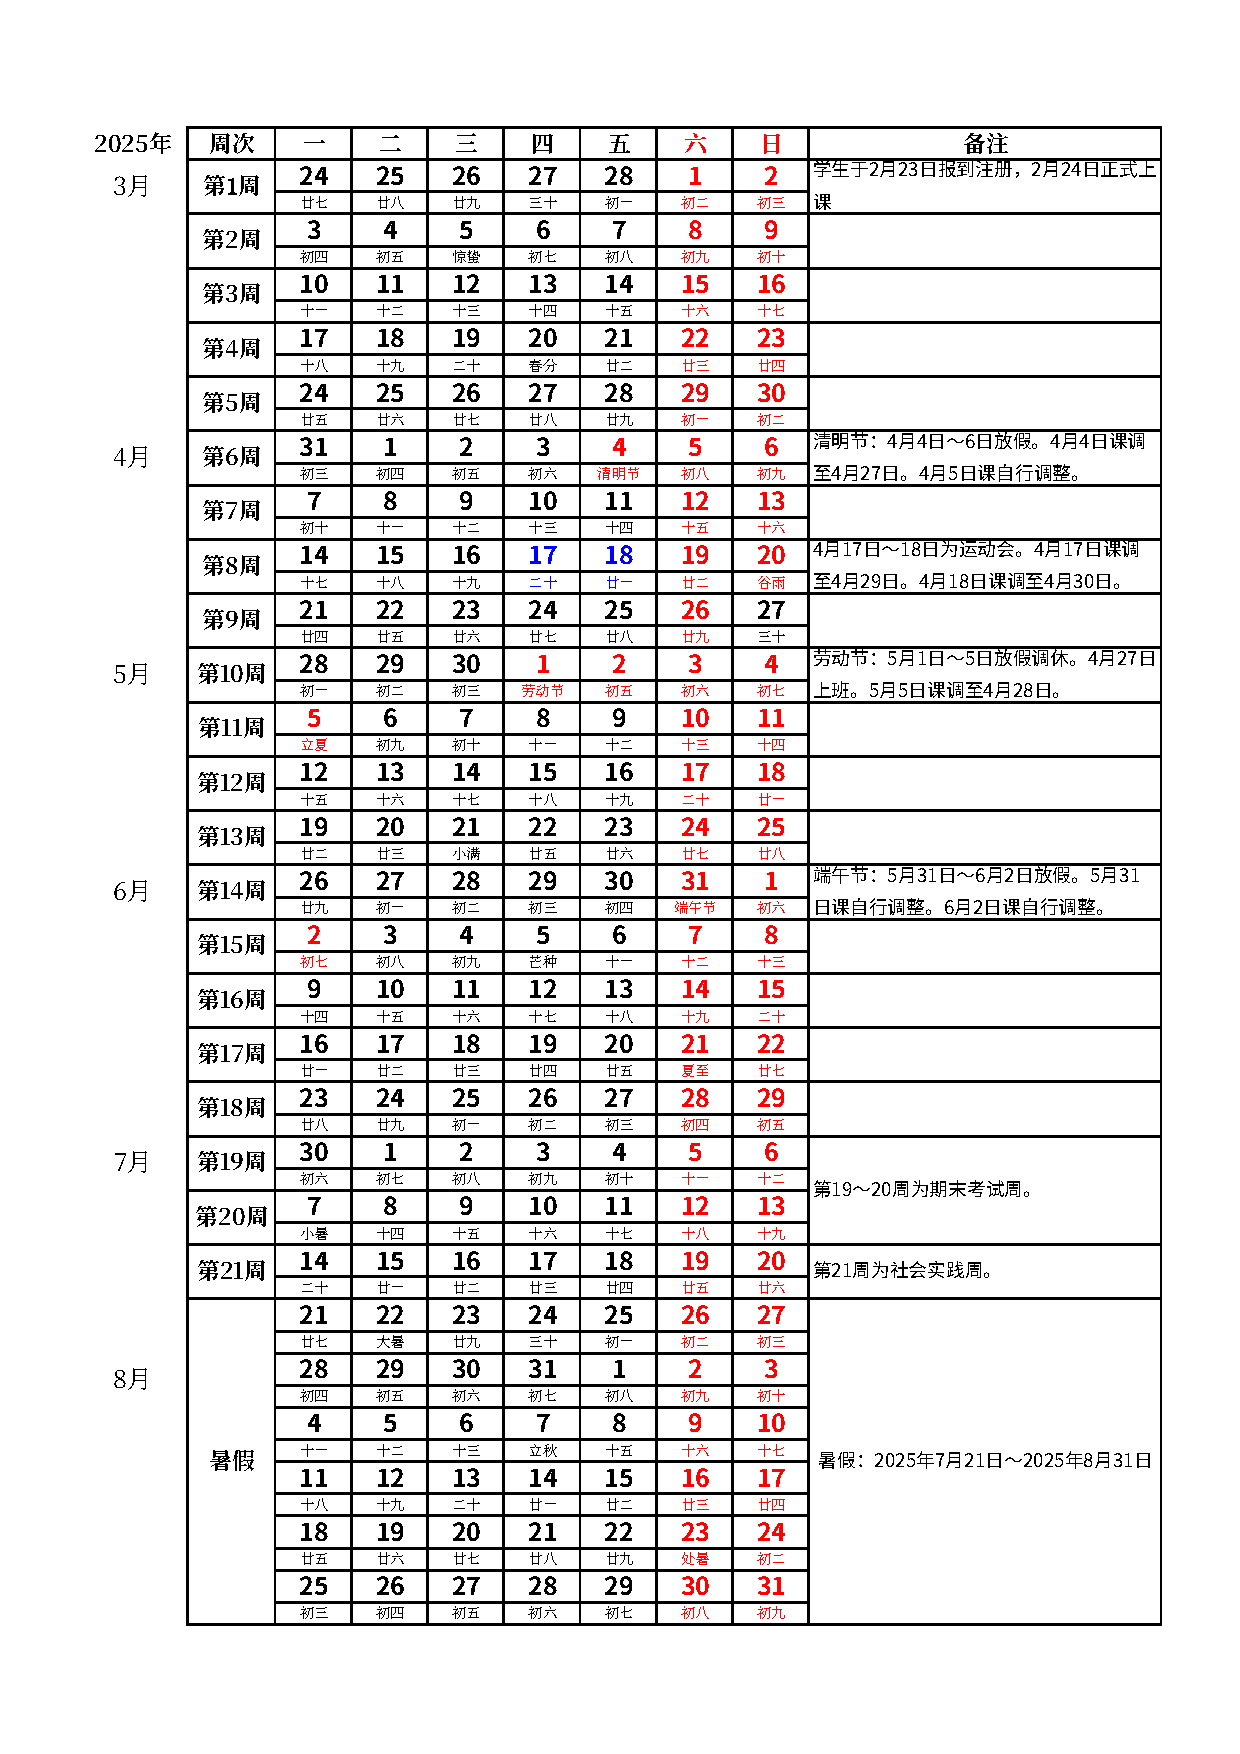
\includegraphics[width=\textwidth]{resources/date/calender.pdf}
}%校历

% 新生入校指南

\chapter[新生报道]{新生报道}

% 入学准备
\section[入学准备]{入学准备}

\subsection[必要证件及物品]{\uuline{必要证件及物品}}
\begin{enumerate}
    \item \textbf{\uuline{录取通知书}}\footnotemark(必须带!!!)
          \footnotetext{录取通知书共两份,一份自行留存收藏,一份上交。}
    \item 身份证原件及其正反面复印件共4份(建议提前自行复印)
    \item 少量零散现金(100元左右即可)\footnotemark
          \footnotetext{校内各商店、超市、食堂支持微信、支付宝支付,部分支持云闪付;暂不支持数字人民币。}
    \item \textbf{证件照红、蓝、白底,1寸各6张、2寸各4张;以及各电子版}(开学后办理证件,如学生证、图书馆借阅证、社团会员证;各类手续,如团关系转接,学生档案转接,学生会入会申请表,体检报告等均需频繁使用;宿舍门禁系统登记时需要提供白底照片电子版)
    \item \textbf{\uuline{学生档案、团员档案}}(丢失或私自拆封需要补办后入学,切记勿忘勿丢勿拆!)
    \item \textbf{手机及配件}(充电器,充电宝,耳机,4~6根数据线〔长度在0.5m~1.5m均可〕)
    \item U盘(方便在校期间打印文件,避免异地登录QQ、微信泄露信息〔8G左右即可〕)
    \item \textbf{常备药物}(碘酒,创可贴,医用棉签,感冒灵,布洛芬,维生素,藿香正气水,止泻药,止咳药,跌打损伤药等)\textbf{\uuline{症状严重务必及时前往校医院就医,切勿自行用药耽误正规治疗}!}
\end{enumerate}

\subsection[选带证件及物品]{选带证件及物品}
\begin{enumerate}
    \item 户口本复印件1份,户口本本人页复印件4份\footnotemark
          \footnotetext{仅少部分院系要求报到时携带,具体要求以录取通知书为准。}
    \item 高考准考证、成绩证明页面的打印版\footnotemark
          \footnotetext{若录取通知书丢失,可通过以上材料证明身份。\label{lost_offer}}
    \item 相机以及配套储存卡、读卡器(⚠贵重物品,请妥存)
    \item \textbf{笔记本电脑}(班长团支、学生会及社团成员必需,其他同学按需)
    \item 平板\footnotemark
          \footnotetext{按照既往经验,有$\frac{1}{4}$左右的同学刷剧追番玩游戏的频率远超学习。}
    \item 备用眼镜、镜布及镜盒
    \item 病历本、住院证明等(仅因病无法参加军训者必备,详见\uline{\ref{exercise_unattend}})
\end{enumerate}

\subsection[推荐生活用品]{推荐生活用品}

\subsubsection[日用品]{日用品}
\begin{enumerate}
    \item 驱蚊花露水、风油精(严禁使用蚊香及电蚊香以防火灾)
    \item 洗面奶、护手霜、防晒霜等护肤品(不宜过多)
    \item 雨伞(2把,⚠易丢)
    \item 洗衣液/洗衣皂/洗衣粉及肥皂盒(建议带盖)、柔顺剂、消毒液
    \item 1.5L~2L的保温小水壶(冬天教学楼饮水机会上冻,提前接热水去自习好一些)
\end{enumerate}

\subsubsection[宿舍用品]{宿舍用品}
\begin{enumerate}
    \item 腰带(军训服尺码偏大)
    \item 袜子、鞋垫、内衣内裤和夏秋季换洗衣物(袜子至少10双,内衣内裤至少6套以免背阴面宿舍阴天无法及时晾干)
    \item 毯子或空调被(可以在录取通知书中查看本年度的配套被褥\footnotemark 价格,用料和质量都比较实在,据自身需求选订选带)
          \footnotetext{一般含夏被,冬被,褥子,枕芯,蚊帐,暖水瓶,塑料盆各一个;被套,床单,枕套,枕巾各两套;订购后会直接在开学时放到宿舍内,订购教程详见\uline{\ref{freshman_query}}。}
    \item 凉席、床垫\footnotemark(出汗严重或睡眠有特殊需求同学可自行选带)
          \footnotetext{宿舍床铺相对硬。}
    \item 蚊帐(已含于配套被褥中。注意:因四角支撑杆可能不全甚至全无,上铺的同学挂蚊帐比较困难;下铺相对方便。如有相关需求可前往校园周边五金店购买相关配件)
    \item 小锁(1把,用于锁柜子)
    \item \textbf{插排、转换器}(宿舍壁插数量少,刚需转换器;为确保安全,推荐购买公牛等知名品牌产品)
    \item 小台灯或手电筒(可用作考前熬夜学习或突然断电的应急措施)
    \item 衣服撑子、衣服夹子、粘钩(用于晾衣服,衣服撑子10个左右,夹子建议大小均有,被子夹6个,小夹子10个左右,粘钩有无均可)
    \item \textbf{几个干净的大型快递纸箱}(因学校的柜子比较脏且容易掉灰,可以先裁开纸箱子铺到自己的柜子里面再放置物品、衣物等以免弄脏)
    \item 樟脑球3个(不宜过多,放在柜子里以防生虫或衣物因为长期阴天而发霉)
\end{enumerate}

\subsection[学习用品]{学习用品}
\begin{enumerate}
    \item 书包(1个,仅用于上集体课)
    \item 手提袋子(1个,要求是耐脏便宜结实,当作书包用,仅用于实验课\footnotemark)
          \footnotetext{解释说明详见\uline{\ref{schoolbag}}。}
    \item 红蓝铅笔(中华牌很好,相对不容易断。医学实验课上全都是红蓝铅笔绘图)
    \item 订书机及订书钉或回形针(少用,\sout{但用一次头疼一次,因为很少有人有……})
    \item 美工刀,剪刀,胶水,双面胶,透明胶(拆快递、贴证件照常用)
    \item 记号笔(给课本封面写名字,课本也很容易丢)
    \item 4/6级英语考试单词书与练习题(4级6级基本都属于考研基础了,\sout{但愿大家能用上吧,不过\linebreak[3]二手书摊经常能买到全新的二手书,可见很多人都没怎么学})
\end{enumerate}

\subsection[相关注意事项]{相关注意事项}
\begin{enumerate}
    \item \textbf{\uuline{学校主要使用QQ进行联系以及官方通知的下发},且无“勤工俭学部”“兼职部”等学生会部门和社团,如遇类似组织推荐兼职请务必谨慎!}社团详情参见\uline{\ref{community_summary}},若不确定可联系本班班长或教师确认,谨防上当受骗!
    \item 安卓手机信号强度在学校停电时相对强(新生入学期间因违规电器导致跳闸频繁)
    \item 充电宝、充电器建议买名牌产品,杂牌劣质产品易出现用电事故;曾因杂牌劣质充电器短路导致多次宿舍全楼大跳闸
    \item 小台灯应当可充电或使用电池供电,以免停电期间无法使用
\end{enumerate}%入学准备
% 入学报到
\section[入学报到]{入学报到}

\subsection[地址与快递]{\uuline{地址与快递}}
\subsubsection[浮烟山校区]{浮烟山校区}
地址:山东省潍坊市潍城区望留街道宝通西街7166号山东第二医科大学浮烟山校区

快递地址:与学校地址相同

邮编:261053

取快递/寄快递:菜鸟驿站(宿舍楼\#12正北方约70米处,位置参见\hyperref[map_fuyanshan_holistic]{此处}地图)\footnotemark
\footnotetext{营业时间:08:00~20:00。}

\subsubsection[虞河校区]{虞河校区}
地址:山东省潍坊市奎文区广文街道胜利东街4948号山东第二医科大学虞河校区

快递地址:与学校地址相同

邮编:261042

取快递/寄快递:北门菜鸟驿站(在校内,位置见\hyperref[map_yuhe_holistic]{此处})、东门菜鸟驿站(详见\hyperref[common_locations_yuhe]{此链接})\footnotemark
\footnotetext{营业时间:08:30~19:00(北门),08:00~19:30(东门)。}

\subsection[报到时间]{报到时间}
详见本人录取通知书

\subsection[浮烟山校区报到流程]{浮烟山校区报到流程}
\begin{enumerate}
    \item \textbf{\uuline{在“山东第二医科大学学生之家”公众号进行预报到},并查询自己的宿舍编号、学号、班级、学院等信息}\footnotemark(教程详见\hyperref[freshman_query]{此处})
          \footnotetext{公众号查询入口开放日期约为8月20日前后,每年不一。}
    \item 通过学校通知、各级学生会、贴吧或频道创建的官方群内指引或者等待各位带班学长学姐加好友后进入班级群\footnotemark
          \footnotetext{若未能寻找到自己的班级,也可在报到时通过带班学长学姐加入班级官群。}
    \item 根据\hyperref[goto_school]{此处}的指引前往山东第二医科大学(浮烟山校区)北校门,在志愿者\footnotemark 的带领下先前往宿舍一楼(各宿舍楼位置见\hyperref[map_fuyanshan_holistic]{此处}),在宿管阿姨处领取宿舍钥匙并登记信息
          \footnotetext{注意,\textbf{男女宿舍不互通},请尽量找相同性别的志愿者帮忙;浮烟山校区在新生报到时允许家长入校参观、帮助搬运行李,具体时间及相关政策详询学校。}
    \item 暂时放置行李物品,进行物品的初步整理
    \item 携带本人身份证件、录取通知书\footnotemark 及中性笔一只,前往杏林路D区方位(位置参见\hyperref[map_fuyanshan_holistic]{此处})
          \footnotetext{录取通知书丢失处理办法见此\hyperref[lost_offer]{此处}。}
    \item 在公安设置的身份核验处查验自己的身份证\footnotemark 信息
          \footnotetext{身份证丢失或失效请立即在学校110警务处申请临时身份证。}
    \item 根据杏林路西侧的指示牌寻找自己班级的带班学长、学姐报到并签字,他们将指引你完成接下来的报到流程\footnotemark
          \footnotetext{如果前往学校的时间过晚或未能及时购票,可前往学院官网,通过官网最下方的联系方式咨询本学院教师及教务处解决方案,否则将视为自动放弃入学资格;按照往年惯例,未能及时登记报到的同学将统一补齐相关记录。}
    \item 返回宿舍或前往菜鸟驿站领取并整理自己的被褥等个人物品
\end{enumerate}%入学报到
% 交通指引

\section[交通指引]{交通指引}
\label{goto_school}
\subsection[火车(高铁)]{火车(高铁)}
起点:家乡的火车站

终点:优选“潍坊站”,其次“潍坊北站”(因北站距离学校较远,公交线路\uref{bus}{见此})

提示:在购票窗口出示你的录取通知书(不可使用复印件)后,高铁打七五折,火车票五折

出站口选择:
\begin{enumerate}
    \item 潍坊站:如需学校迎新官方接送或乘坐公交请选择“北出站口”,打车请往“南出站口”;需要前往虞河校区请走“北出站口”
    \item 潍坊北站:请先乘25或106路公交至潍坊站,再按上面的指引前往
\end{enumerate}

\subsection[大巴(公交)]{大巴(公交)}

\subsubsection[官方接站]{官方接站}
学校每年都会在潍坊站(含潍坊北站)、潍坊长途汽车总站设立“山东第二医科大学新生接待处”,有专车接送新生到浮烟山校区,运营时间为07:00~17:00。接待点内的工作人员均会佩戴山东第二医科大学校徽及其他相关标识

\subsubsection[自行前往]{自行前往}
\label{bus}
\begin{enumerate}
    \item 浮烟山校区
          \begin{enumerate}
              \item 在潍坊站下火车的同学可从“北出站口”出站,乘坐69、71或101路公交车在“山东第二医科大学北门”站下车(预计30~50分钟左右)
              \item 在潍坊北站下火车的同学可先乘坐25或106路公交车前往火车站(潍坊站),再以上述方式前往报到(潍坊北站至潍坊站约需2小时)
          \end{enumerate}
    \item 虞河校区
          前往虞河校区可从“北出站口”出站,乘坐13路或75路公交车,在“鸢飞路胜利街路口北”站下车(预计20~30分钟左右)
\end{enumerate}

\subsection[出租车]{出租车}
浮烟山校区:建议乘坐正规出租车,地点为“山二医新校区北门”,正规出租车打表价格约25元(预计时间20~25分钟)

虞河校区:地点为“山二医老校区(虞河校区)北门”,打表价格约20元(预计时间15~20分钟)

\subsection[浮烟山校区新生报到提示]{浮烟山校区新生报到提示}
浮烟山校区南门提供摆渡车(观光车)且有志愿者帮助运送行李,但因距离宿舍较远、搬运行李不便,推荐走北门报到(报到结束后,可乘观光车在南门处拍照留念)%交通指引

% 军训
\section[军训]{军训}

\subsection[军训概况]{军训概况}
\begin{enumerate}
    \item 军训时间:3周,报到后马上开始
    \item 内容\footnotemark:站军姿、蹲下、跨立、齐步走、原地踏步、齐步跑、踢正步、坐马扎
          \footnotetext{不打靶、不摸枪;少数同学会参与战术方阵,女生有擒敌拳。}
    \item 地点:多数在杏林路树荫下军训(一般晒不着,但仍然建议多备防晒霜)
    \item 教官:按往年情况,一般由部队官兵担任
    \item 着装:穿着统一的军训套装\footnotemark
          \footnotetext{同被褥套装订购教程请看\uref{freshman_query}。含T恤、外套、裤子(很肥)、腰带(扎在外套外面,需另备一条腰带以免掉裤子)、鞋子(底薄、磨脚,推荐鞋子大一号多垫几双鞋垫)和马扎(军训完不要扔,考试月背书很好用)。}
    \item \textbf{如果因为身体原因不能参加军训,需要提前拿病历、住院证明等材料前往校医院开具相关证明\label{exercise_unattend}}(位置见\uref{map_fuyanshan_holistic})
    \item 若出现身体不适要及时向教官报告,较严重的可申请前往校医院或附属医院进行详细检查
    \item \sout{如果顺拐和左右不分情况极其严重的,可以早早申请成为“飞虎队”\footnotemark 的一员}
          \footnotetext{谐音梗,音同废物队;是对严重顺拐同学的无恶意调侃。}
    \item 特点:军训期间时间紧、任务重,少有可以自由安排的时间
    \item 注意:\textbf{\uuline{可能出现长时间阴天}},因此推荐多带袜子、内裤、内衣、T恤以避免一件衣服穿一周(\sout{熏死啦,想想就头大})、袜子晾干以后变得硬邦邦的(\sout{长蘑菇了都})的悲伤结局
\end{enumerate}

\subsection[军训作息时间表]{军训作息时间表\footnotemark}
\footnotetext{以往届作息为例,具体以各学院安排为准。}
\begin{table}[H]
    \centering
    \begin{tblr}[
            theme = {no-caption},
        ]{
            cells = {c,m},
            hlines,
            vlines,
        }
        05:30        & 起床 & 12:30~14:00 & 午休   \\
        06:00~07:00 & 早操 & 14:00~17:30 & 集训   \\
        07:00~07:50 & 早餐 & 17:30~18:30 & 晚餐   \\
        07:50~11:00 & 集训 & 19:00~21:00 & 晚自习 \\
        11:00~12:30 & 午餐 & 23:00        & 熄灯   \\
    \end{tblr}
\end{table}
%军训

% 费用
\section[费用、ATM与银行卡]{费用、ATM与银行卡}

\subsection[生活费]{生活费}
一般生活费范围约1000~1500元(仅吃饭和购买水果、牛奶等常规生活情景)

\subsection[学费]{学费\footnotemark}
\footnotetext{学费缴费系统使用教程\hyperref[fee_pay]{见此},财务处地址:行政楼1层西侧。}
\subsubsection[一般情况说明]{一般情况说明}
\begin{enumerate}
    \item 学费通常分为四部分\footnotemark
          \footnotetext{详见财务处文件\href{https://cwch.sdsmu.edu.cn/_upload/article/files/47/c4/47b017924d219d29d49dd079335a/f04e22ac-aa91-4c49-bceb-f53280c93164.pdf}{《学分制收费管理办法》}、\href{https://cwch.sdsmu.edu.cn/_upload/article/files/ce/67/093a0208463a8a5bb333e3117fc6/dfb39999-8683-49e7-b8b0-0ed7af8a6150.pdf}{《关于印发山东省高等学校住宿费收费管理办法的通知》}等。}
          \begin{enumerate}
              \item 专业注册学费:不同专业不一,按学年收取
              \item 学分学费:根据各人选修课情况收费,按学期收取
              \item 住宿费:不同校区、楼栋标准不一,按学年收取
              \item 书费:订书方式多样,费用与收费时间均不确定,请以班级群内通知为准
          \end{enumerate}
    \item 依惯例,新生入学时需要进行缴纳第一学期的专业注册学费与住宿费,请按录取通知书说明以及新生预报到系统\footnotemark 的提示进行
          \footnotetext{预报到系统使用教程\hyperref[freshman_query]{见此}。}
    \item 学费的收缴工作在开学后按照学校财务处通知进行,通常以班级为单位进行通知,可开具电子发票
    \item 公费医学生与助学贷款学生无须缴纳专业注册学费、学分学费、住宿费3类费用
    \item 如需申请助学贷款、生源地贷款等有特殊情况的同学详询财务处收费管理科(联系方式详见官网)
    \item 选修课学费按照学分进行收费,所以同一个班的同学学费亦可不同,个人学费以\textbf{“山东第二医科大学财务处”公众号(山东第二医科大学校园统一缴费平台)}中的数据为准
    \item 选修课学分当前规定为1分/100元,多选课多交钱,少选课少交钱(希望大家如果看到了自己希望进一步学习的课程不要吝啬那几百块钱,选课机会只有一次,课程不会重开!)
    \item 此外,一定结合培养方案的要求(见\hyperref[score]{此处})修够学分,\textbf{否则无法毕业}
\end{enumerate}

\subsection[助学项目与困难补助]{助学项目与困难补助}
\subsubsection[助学项目一览]{助学项目一览}
敬请参照山东省教育厅学生资助管理中心\href{https://sdxszz.sdei.edu.cn/Show/7784}{《山东省普通高等学校资助政策简介》}或咨询学校教师
\subsubsection[困难补助一览]{困难补助一览}
详见学校下发的《山东第二医科大学新生报到指南》

\subsection[ATM]{ATM\footnotemark}
\footnotetext{根据业务动态调整,详情见各银行官网。}
\begin{enumerate}
    \item 工商银行:教学楼E区,靠近杏林路侧
    \item 邮政银行:中和广场,A103对过
\end{enumerate}

\subsection[银行卡]{银行卡}
学校统一为各位同学办理一张中国工商银行卡,在入学后发放。该卡包含学生个人信息,将用于大学生活中用于奖助学金等其他费用的发放

\textbf{\uuline{严禁出借银行卡,否则可能导致违法犯罪!!!}}
%费用相关

% 新生常见问题
\section[常见问题]{常见问题}
\begin{enumerate}
    \item 第一临床医学院与临床医学院的区别\\
          “第一临床医学院”为学校与第一附属医院(潍坊市人民医院)合署招生,实习与见习将定向至该医院。新生将随机分配至临床医学院与第一临床医学院
    \item 宿舍分配\label{random_allocation}\\
          无规律,宿舍以专业为单位随机分配宿舍楼、班内宿舍按姓氏顺序分配,与录取分数无关;宿舍床位为自行挑选,如有不妥可在辅导员知情同意的情况下宿舍内协商解决
\end{enumerate}
%其他常见问题%新生报道

% 浮烟山目录

\chapter[浮烟山校区]{浮烟山校区}

% 校区概况
\section*{校区概况}
\begin{enumerate}
    \item 学校大部分学院、年级、部门所在
    \item 有南、北、西、东北三个校门,按时关门、封闭式校园\footnotemark
          \footnotetext{西门不对学生开放。外部外卖不允许进校园,校内有商家配送的校内外卖。}
    \item 学校宿舍条件较虞河校区好,有独卫,部分宿舍有独浴,每层有饮水机;按时熄灯、按时关门
    \item 教学建筑:教学楼4座,实验楼4座,办公楼2座,书院1座
    \item 生活建筑:有操场2个,餐厅2个,服务中心2个,水房1个,文体中心1座(含游泳馆、篮球馆、乒乓球馆、羽毛球馆、健身馆、旱地冰球场等),操场2个,网球场1处,篮球场数个,菜鸟驿站1座,校医院1座、隔离方舱数间,小超市2个
    \item 周围基础设施建设完备情况较为一般,大型商超0个,大型连锁快餐店0个,大型游乐场0个,大型电影院0个,集市1处,小吃街1条
    \item 距离市中心约15分钟(出租车)或45分钟(公交)
\end{enumerate}

\begin{tblr}[
        long,
        label = {common_lab_department_fuyanshan},
        caption = {常用位置},
    ]{
        rowhead = 1,
        cells = {c,m},
        row{1} = {font=\bfseries},
        vlines,
        hlines,
        hline{1-2,9,16}= {-}{1pt},
    }
    地点(俗称)   & 位置(简称)   & 提示                             \\
    110警务中心    & 敏行楼C座1楼北 & 无法补办身份证件                 \\
    财务处         & 办公楼1楼西    & 请注意业务办理时间               \\
    教务处         & 办公楼3楼西侧  & 不同科室位置不同,请提前电联咨询 \\
    学生档案室     & F区2楼         & 需网上预约或提前电联咨询         \\
    校医院         & 仁和山         &                                  \\
    公寓管理委员会 & 2号公寓东南侧  & 需预约                           \\
    餐厅办公室     & 餐厅2层东侧    & 需预约                           \\
    解剖实验室     & 敏行楼B座西南  & 系解、局解合用                   \\
    病生实验室     & 敏行楼A座东北  & 药理、生理合用                   \\
    微生物实验室   & 敏行楼A座北    & 化诊、寄生虫、基础医学共用       \\
    遗传学实验室   & 敏行楼A座北    & 免疫、细胞、病理合用             \\
    流行病实验室   & 致远楼A座      &                                  \\
    临床技能学     & 临床技能中心   & 部分实验室需要从敏行路一侧进入   \\
    统计学实验室   & 图书馆1楼      &
\end{tblr}

%总述
% 地图

%\newpage
\section[地图]{地图\footnotemark}
\footnotetext{参考及声明:整体地图——校宣传部,教学楼地图——临床医学院2021级学工办,附院浮烟山院区地图——临床医学院。其他版权声明见\uline{\ref{copyright}}。}

\subsection[教学楼内部(浮烟山校区)]{教学楼内部(浮烟山校区)}
\begin{figure}[H]
    \centering
    %\vspace{6em}
    \includegraphics*[width=0.99\textwidth]{resources/map/浮烟山校区教学楼.pdf}
    \label{map_fuyanshan_teach_building}
\end{figure}

\newpage
\subsection[敏行楼内部(浮烟山校区)]{敏行楼内部(浮烟山校区)}
因敏行楼门牌号在各楼层不对称、不对应,故本图并不十分精确,仅用做示意。实地寻找实验室请根据教师提供的门牌号查看地图,在对应位置的附近寻找(X代表楼层,取值范围为1~4)
\begin{figure}[H]
    \centering
    \includegraphics*[height=0.9\textheight]{resources/map/浮烟山校区敏行楼_矢量.pdf}
    \label{map_fuyanshan_minxing}
\end{figure}

\newpage
\subsection[整体(浮烟山校区)]{整体(浮烟山校区)}
\begin{figure}[H]
    \centering
    \includegraphics*[height=0.9\textheight]{resources/map/浮烟山校区简图.pdf}
    \label{map_fuyanshan_holistic}
\end{figure}

\newpage
\subsection[整体(附院浮烟山院区)]{整体(附院浮烟山院区)}
\begin{figure}[H]
    \centering
    test
    %\includegraphics*[height=0.9\textheight]{resources/map/浮烟山校区简图.pdf}
    \label{map_affiliated_hospital_fuyanshan}
\end{figure}

\newpage%地图
% 宿舍
\section[宿舍条件]{宿舍条件}

\subsection[整体情况介绍]{整体情况介绍}
\begin{enumerate}
    \item 绝大多数的宿舍为6人间,上下床\footnotemark(各床铺靠墙侧均有1插座,可接插排),配备桌子(桌洞8个)一张,书桌(理论可坐3人但空间紧张,常2人,含6个小书架)一张,有柜子(常为8个),垃圾桶,洗漱池,空调,电风扇,暖气片,烟雾报警器等宿舍基本设施
          \footnotetext{床铺尺寸为:长200cm,宽90cm;被子尺寸为:长210cm,宽148cm。}
    \item 柜子\footnotemark 一般为8个,6人各选一个柜子,剩下两个公用
          \footnotetext{空间尺寸参数大致如下:宽62cm,高59cm,深97cm(各有1~2cm误差)。}
    \item 具有独立卫生间
    \item 部分女生宿舍的卫生间内有浴室,可直接在卫生间内淋浴;其他同学可以在本楼层小公共澡堂(有2个毛玻璃隔间,有门帘,无需预约)或者一楼的大公共澡堂(不透明隔间,有门帘,需软件预约)洗澡(教程见此\uline{\ref{shower_software_f}})
    \item 洗衣机位于每层楼的公共洗漱间内(教程见此\uline{\ref{washing_machine_f}})
    \item 烘干机位于每栋楼1层公共洗漱间内(教程见此\uline{\ref{dry_machine}})
    \item 吹风机位于每层楼的公共厕所旁(教程见此\uline{\ref{hair_drier}})
    \item 大一期间,院学生会每周不定时抽查是否存在夜不归宿情况
    \item 空调采用单独线路供电,不受断电熄灯控制(全楼断电等特殊情况除外),需另外缴费(使用教程参见\uline{\ref{air_control}})
    \item 使用门禁系统刷脸进出宿舍,宿舍楼06:00开门,23:00关门
    \item 每天23:00断电(\textbf{每周六、考试月和每年9月的第一个星期除外})
    \item 宿舍楼提供免费的100℃开水\footnotemark,若对饮水水质要求不高也可直接饮用;否则请前往大学生服务中心〔简称“大服”〕打水处(位置参见\uline{\ref{map_fuyanshan_holistic}})付费接取纯净水
          \footnotetext{饮水机每层一个,位于公共洗漱间内;为自来水烧开;熄灯后停止供应。推荐用于泡面、洗衣、泡脚等用途。}
    \item \textbf{\uuline{宿舍单个插座限电400W,超限将导致全楼停电}}
    \item 除跳闸断电等特殊情况外,其余时间段均有4G及5G信号覆盖,延迟波动较大(15~999$^+$㎳),平均网速1.5~5㎆/s
\end{enumerate}

\subsection[住宿注意事项]{住宿注意事项}
\begin{enumerate}
    \item 是否自带被褥等可按照个人需求决定\footnotemark
          \footnotetext{新生军训期间对于床单的颜色等具有特别要求,详见录取通知书相关说明。}
    \item 宿舍门禁系统将在开学军训期间进行人脸录入,\textbf{\uuline{切忌美颜过度,否则无法识别}}
    \item 无特殊情况\textbf{禁止自挂床帘},特殊需求请找导员开具证明
    \item 宿舍内备有烟雾传感器,\textbf{吸烟将引发报警\footnotemark}
          \footnotetext{若烟雾报警器报警,请立即联系宿舍管理人员或保卫处核实。}
    \item 床上桌等类似的东西建议到学校实际生活1个月以后再决定是否购买(大部分人都用不到,少数同学用来打游戏,\sout{然而身体在床上缩着打游戏超级难受};更少一部分同学用其学习,\sout{该现象\linebreak[3]比彩色大熊猫更加罕见})
    \item 宿舍单个插座的功率限制400W\footnotemark,\textbf{\uuline{吹风机、锅、电暖宝、电水壶、热得快等高功率电器均严\linebreak 禁使用},否则将引起宿舍全楼停电};宿管不定期来查,若被发现将被没收并通报批评、检讨
          \footnotetext{如果接了一个插排,插排的总功率不能超过400W,例如一个67W的手机充电器和2个175W的游戏本电脑就立马跳闸了。}
    \item 如需美化宿舍环境,可通过参加学校统一开展的\textbf{“宿舍文化月”}\footnotemark 以对宿舍进行小幅调整
          \footnotetext{禁止外来装修人员入校、禁止私改电路,详情内容见开学后下发的相关要求。}
    \item 背阴面宿舍的阳台作用极小,\textbf{推荐在楼下晾晒衣物},若只靠阴干,很容易发霉发臭;向阳面无此困扰
    \item \textbf{一旦离开宿舍必须关灯关电关水,若插排未拔将被没收并扣分}
    \item 禁止将正在持续充电的手机、充电宝直接置于被子等密闭、空气无流通的环境中,极不推荐直接将笔记本电脑置于被子上使用,严重影响散热且有着火风险
    \item \textbf{\uuline{为保证他人睡眠,熄灯后严禁使用台灯、手电筒在宿舍内继续学习;更不要制造噪音!}}\footnotemark
          \footnotetext{很多同学难以入睡且睡眠浅,小动静或急速的明暗变化就能被惊醒,请大家务必相互尊重、相互理解。}
    \item 如遇宿舍公用物品(如门锁,门轴,玻璃窗,灯管,水龙头,下水道等)损坏,请直接报修(教程见此\uline{\ref{repair_report}})
    \item 宿舍一层有便民驿站(含针线包、打气筒、简易医药箱),即用即还
    \item 雨伞不得长时间放置于宿舍门外,避免影响正常通行
    \item \textbf{严禁在23:30以后使用洗衣机、烘干机、吹风机或洗澡}
\end{enumerate}

%宿舍
% 生活
\section[衣食购住玩与生活]{衣食购住玩与生活}

\subsection*{特别声明}
\begin{enumerate}
    \item 本文中所有\textbf{“大服”},均为\textbf{“大学生服务中心”}的习惯性缩略称呼;
    \item 本文中所有\textbf{“南街”},均为\textbf{“汇金街”}的习惯性缩略称呼。
\end{enumerate}
\subsection[衣]{衣}
\begin{enumerate}
    \item 大服的2、3层均有服饰商店可自行选购衣物
    \item 推荐网购,也可根据\uref{free_bus}{后文}的公交车信息前往大型商超购置
    \item 部分院系提供自愿的系服购买服务,详见各院系通知
\end{enumerate}

\subsection[食]{食}
\subsubsection*{注意}
\begin{enumerate}
    \item 因文章篇幅原因,本指南仅列举了同学们提及次数较多的部分食物或店铺,敬请谅解;
    \item 下列提及的店铺(食物)均按照空间顺序排列,与好吃程度无关;
    \item 所用名称为同学习惯性称呼,括号内为特别提醒或补充说明。
    \item 上标“㊐”的店铺夏季约06:00开始供应(冬季约06:30);
    \item 上标“㊰”的店铺营业时间最晚可至22:30,其余均在18:30~20:30左右停业;
    \item 上标“㊒”的店铺因装修等原因尚未开业或长期停业(超过一周);
    \item 奶茶/咖啡店、水果店等单独说明。
\end{enumerate}

\subsubsection[杏林餐厅]{杏林餐厅}
杏林餐厅全部三层均有大量食物,大多物美价廉。
\begin{table}[H]
    \centering
    \begin{tblr}[
            theme = {no-caption},
            note{1} = {除餐厅东南侧楼梯外均可到达。},
        ]{
            cells = {c,m},
            cell{1}{1} = {r=3}{},
            cell{4}{1} = {r=3}{},
            cell{7}{2} = {c=4}{},
            vlines,
            hlines,
            hline{1,4,7-Z} = {-}{1pt},
            column{1} = {cmd=\bfseries},
        }
        1层             & 麦西麦乐                                     & 包子水饺$^㊐$        & 牛肉板面 & 兰州拉面         \\
                        & 大米粒儿$^㊐$(油条)                        & 自选菜(稍贵)       & 豆腐脑   & 盒饭(便宜量大) \\
                        & 粥$^㊐$(种类多)                            & 馄饨$^㊐$            & 麻辣烫   & 烤夫王           \\
        2层             & 大骨饭                                       & 麻汁馄饨             & 水饺     & 东北玉米面       \\
                        & 烤鸭饭(瓦罐汤)                             & 铁板炒饭(量大管饱) & 米线     & 清真窗口         \\
                        & 馋嘴鱼                                       & 自选水饺             & 茶拌饭   & 略               \\
        3层\TblrNote{1} & 略(较贵。有包间、舞台、音响等,需提前预约) &                      &          &
    \end{tblr}
\end{table}

\subsubsection[大服]{大服}
大服有大量商家提供多种食物,大部分的价格较食堂稍高。
\begin{tblr}[
        long,
        theme = {no-caption},
    ]{
        cells = {c,m},
        cell{1}{1} = {r=3}{},
        cell{1}{2} = {r=2}{},
        cell{4}{1} = {r=2}{},
        cell{4}{2} = {r=2}{},
        vlines,
        hlines,
        hline{1,4,Z} = {-}{1pt},
        hline{3} = {2-6}{0.8pt},
        column{1} = {cmd=\bfseries},
    }
    1层   & 内           & 金小麵$^㊐$(锅贴) & 自选菜                 & 陕西面馆        & 馋嘴鱼        \\*
          &              & 新疆炒米粉          & 肠粉                   & 肉夹馍$^㊰$     & 冒菜          \\*
          & 外           & 烧烤$^㊰$           & 砂锅$^㊐$(火烧|豆脑) & 大饼卷一切$^㊰$ & 速食主义$^㊐$ \\
    --1层 & $\backslash$ & 兰李于              & 自选菜                 & 酸菜鱼          & 螺狮粉        \\*
          &              & 烤鸡架              & 宽巷面馆               & 馋嘴鱼          & 略
\end{tblr}

%\newpage
\subsubsection[汇金街]{汇金街}
出学校南门,往东一个路口。有大量的饭店,价格大多较市里相对高昂,部分味道一般。
\begin{table}[H]
    \centering
    \begin{tblr}[
            theme = {no-caption},
        ]{
            cells = {c,m},
            hline{1,Z}= {-}{1pt},
            vlines,
            hlines,
        }
        满江红   & 暖溢水饺(相对平价) & 木南王府 & 小四川烧烤           \\
        志科全驴 & 炖大鹅               & 生炖羊茬 & 幸福餐厅(平价量大)
    \end{tblr}
\end{table}

\subsubsection[水果店]{水果店}
\begin{table}[H]
    \centering
    \begin{tblr}[
            theme = {no-caption},
        ]{
            cells = {c,m},
            hline{1-2,Z}= {-}{1pt},
            hlines,
            vlines,
            row{1} = {cmd=\bfseries},
        }
        习惯称呼      & 地点                          & 种类 & 新鲜 & 价格 \\
        餐厅南水果店  & 餐厅正南侧入口                & 较多 & 较好 & 略高 \\
        餐厅西水果店  & 餐厅正西侧入口                & 较少 & 一般 & 一般 \\
        大服水果店    & 大服西南侧                    & 最多 & 一般 & 最高 \\
        中和/大服超市 & \uref{market_fuyanshan}{见此} & 最少 & 一般 & 一般
    \end{tblr}
\end{table}


\subsubsection[奶茶/咖啡店]{奶茶/咖啡店}
\begin{table}[H]
    \centering
    \begin{tblr}[
            theme = {no-caption},
        ]{
            cells = {c,m},
            cell{1}{1}={r=2}{},
            cell{3}{1}={r=2}{},
            hlines,
            vlines,
            hline{1,3,Z}= {-}{1pt},
            hline{4} = {2-6}{0.8pt},
            column{1} = {cmd=\bfseries},
        }
        食堂 & \textbf{蜜雪冰城} & 臻茶              & 沪上阿姨   & 阿水大杯茶        & 麦克风       \\
             & 超级奶爸          & 小度              & 冰雪岛     & \textbf{瑞幸咖啡} & $\backslash$ \\
        大服 & 1层/--1层         & \textbf{茶百道}   & 益禾堂     & \textbf{幸运咖}   & 归臻咖啡     \\
             & 2层               & \textbf{库迪咖啡} & 遇觅烧仙草 & 手打冰沙          & $\backslash$ \\
    \end{tblr}
\end{table}

\subsection[购]{购}
\begin{table}[H]
    \centering
    \label{market_fuyanshan}
    \begin{tblr}[
            theme = {no-caption},
        ]{
            cells = {c,m},
            hline{1-2,5}= {-}{1pt},
            hlines,
            vlines,
            row{1} = {cmd=\bfseries},
        }
        习惯称呼      & 地点           & 物品                                     \\
        大服超市$^㊰$ & 在大服正中央   & 日用品,零食,饮料,手套,头套,作业本等 \\
        中和超市      & 中和广场       & 日用品(少),零食,饮料,作业本等       \\
        餐厅超市      & 餐厅西北侧入口 & 餐巾纸、零食、饮料等
    \end{tblr}
\end{table}

\subsection[玩]{玩}
\begin{enumerate}
    \item 多数同学常通过步行前往南街,有KTV、电影院等娱乐场所
    \item 汇金街每逢农历初三、初八、十三、十八、廿三、廿八有集
    \item 前往市区的公交线路详情参见\uref{free_bus}{公交信息与免费乘车指南}
    \item 文体中心(位置参见\uref{map_fuyanshan_holistic}{此处})内有羽毛球馆、篮球馆(两者互斥)、健身房,还有\textbf{游泳馆}等\footnotemark
          \footnotetext{具体收费标准及预约方式见\uref{sports_center_book}{下文},开放时间见下表。}
\end{enumerate}

\begin{tblr}[
        long,
        label = {sports_center_operating_hours},
        caption = {文体中心开放时间},
        note{1} = {仅限校内,校外政策详见公众号或咨询工作人员;具体政策请以学校通知为准。},
    ]{
        cells = {c,m},
        rowhead = {2},
        row{1} = {font=\bfseries},
        column{1} = {font=\bfseries},
        cell{1,3,12}{1} = {r=2}{},
        cell{1}{2} = {c=3}{},
        cell{3}{3} = {c=2,r=5}{},
        cell{5}{1} = {r=3}{},
        cell{8}{1} = {r=4}{},
        cell{8,10}{2} = {r=2}{},
        cell{8-11}{3} = {c=2}{},
        cell{12}{2} = {c=2,r=2}{},
        vlines,
        hlines,
        hline{1,3,8,12,Z} = {-}{1pt},
        hline{2,10} = {2-4}{0.8pt},
        hline{5} = {1-2}{1pt},
    }
    开放项目 & 春夏季营业时间                                   %
    \TblrNote{1}                                                \\
             & 周一至周四     & 周五         & 周末及法定节假日 \\
    健体中心 & 11:45~13:45   & 08:00~21:00                    \\*
             & 18:00~21:00   &                                 \\*
    羽毛球馆 & 08:00~09:30   &                                 \\*
             & 12:00~13:30   &                                 \\*
             & 18:00~21:00   &                                 \\
    游泳馆   & 12:00~14:00   & 09:00~11:00                    \\*
             &                & 12:00~14:00                    \\*
             & 18:00~20:00   & 15:00~17:00                    \\*
             &                & 18:00~20:00                    \\
    乒乓球馆 & 18:00~20:00   &              & 08:00~12:00     \\*
             &                &              & 14:00~20:00
\end{tblr}

\subsection[住]{住}
\begin{enumerate}
    \item 宾馆:南街提供大量宾馆、客房等
    \item 自习室:南街部分宾馆提供通宵自习服务
    \item 出租房:附近小区有较多房屋出租\footnotemark
          \footnotetext{须在学校办理走读手续后才可在外居住。}
\end{enumerate}

\subsection[自提点]{自提点}
\begin{tblr}[
        long,
        theme = {no-caption},
    ]{
        cells = {c,m},
        cell{2}{1} = {r=2}{},
        cell{4}{1} = {r=2}{},
        row{1} = {font=\bfseries},
        rowhead = {1},
        vlines,
        hlines,
        hline{1-2,4,Z} = {-}{1pt},
    }
    类别     & 地点           & 显示名称                 \\
    美团优选 & 中和移动营业厅 & 山二医美团优选移动       \\*
             & 9号宿舍楼      & 山二医九号楼群内免费送货 \\\linebreak[2]
    多多买菜 & 中和移动营业厅 & 潍医多多买菜移动营业厅   \\*
             & 9号宿舍楼      & 山二医九号楼自提
\end{tblr}

\subsection[其他生活常用地点]{其他常用地点}
\begin{tblr}[
        long,
        caption = {其他常用生活地点详表},
        label = {common_locations_fuyanshan},
        note{1} = {清晰度较“学生印务”略高,少量打印时价格略高。},
        note{2} = {仅大服北侧楼梯可前往,健身卡收费详情咨询工作人员,与文体中心健身房不同。},
        note{3} = {注意,该邮局无信件投递及接收业务。},
    ]{
        cells = {c,m},
        rowhead = {1},
        row{1} = {font=\bfseries},
        column{1} = {font=\bfseries},
        cell{2}{1} = {r=17}{},
        cell{19}{1} = {r=3}{},
        cell{22}{1} = {r=5}{},
        vlines,
        hlines,
        hline{1-2,19,22,Z} = {-}{1pt},
    }
    地点     & 习惯称呼                & 位置           & 功能                                     \\
    大服     & 厕所                    & --1层东北      & 略                                       \\*
             & 联通营业厅              & 1层超市旁      & 联通业务办理                             \\*
             & 药店、牙科诊所          & 2层西北        & 买药、看牙、\textbf{冷藏药品}            \\*
             & 智慧驾校                & 2层西北        & 驾考咨询、驾校报名                       \\*
             & 理发店(三家)          & 2层            & 烫染剪发                                 \\*
             & 复印店(两家)          & 2层            & \textbf{打印复印扫描、证件照}、 复习资料 \\*
             & 电信营业厅              & 2层            & 电信业务办理                             \\*
             & 移动业务咨询处          & 2层东          & 移动业务咨询                             \\*
             & 广电营业厅              & 2层北          & 广电业务办理                             \\*
             & 干洗店                  & 2层东          & 干洗、实验服购买、配钥匙                 \\*
             & 裁缝店                  & 2层东南        & 改衣                                     \\*
             & 维修店                  & 2层东南        & 手机电脑维修、配件购买                   \\*
             & 联想服务中心            & 2层西          & 维修检测、配件购买                       \\*
             & \textbf{办公室}         & 2层东北        & 办水卡、充值退卡                         \\*
             & 大服健身房 \TblrNote{2} & 3层            & 运动健身、办理会员卡                     \\*
             & 台球厅                  & 3层            & 打台球                                   \\*
             & 彩购师                  & 3层            & 衣物与饰品购买                           \\
    中和广场 & 学生印务                & A106对过       & 打印复印扫描、\textbf{复习资料、二手书}  \\*
             & 移动营业厅              & A104对过       & 移动业务办理                             \\*
             & 酷跑文印社\TblrNote{1}  & A103对过       & 打印复印扫描                             \\
    其他     & 证件照                  & B207旁         & \textbf{证件照}、特殊复印(80g/120g纸)  \\*
             & \textbf{证明打印}       & D105旁         & \textbf{学籍证明、成绩证明}等            \\*
             & 自助打印                & 餐厅北侧       & 打印                                     \\*
             & 二手书买卖              & 大服西北角     & \textbf{二手书}(大量)                  \\*
             & 邮局                    & 餐厅西北侧入口 & 学校纪念品购买 \TblrNote{3}
\end{tblr}

%校园生活各方面%浮烟山章节
% 虞河校区目录

\chapter[虞河校区]{虞河校区}

% 校区概况
\section*{校区概况}
\begin{enumerate}
    \item 仅有部分专业的部分年级
    \item 有北、东两个校门、一个通向眼科中心的小门,开放式校园\footnotemark (禁止共享单车入内)
          \footnotetext{北门24小时开放,东门对行人开放时间为06:00~19:00,通向眼科中心的小门开放时间为06:00~19:00,另有一个极少关闭的小门通往南面的家属院。}
    \item 宿舍条件较差,无独卫独浴、限电(但不停电)、仅单数楼层有饮水机,宿舍按时关门
    \item 教学建筑:教学楼3座,实验楼1座,校史馆1座;教室较小,仅1楼有饮水机
    \item 生活建筑:操场0个,篮球场1个(非标准),餐厅1个,浴室(地下)男女各一,小超市2个
    \item 接近市中心,周围可供饮食、娱乐、购物等,\textbf{应有尽有}
    \item 学校内建有整形医院、生殖中心、眼科等科室,人员流动频繁;请及时锁门以免失窃
    \item \textbf{其他未提及的事项敬请参见浮烟山校区相关内容}
\end{enumerate}

\begin{tblr}[
        long,
        label = {common_locations_yuhe},
        caption = {常用位置},
    ]{
        rowhead = 1,
        cells = {c,m},
        row{1} = {font=\bfseries},
        hline{1-2,7,Z}= {-}{1pt},
        vlines,
        hlines,
    }
    地点(俗称)     & 位置(简称)      & 提示                               \\
    物业维修中心     & 警务中心西20米    & 需提前在宿管处填写报修单据         \\
    餐厅超市(打印) & 餐厅2楼           & 可打印复印、买水果零食等           \\
    地下便利店       & 3号楼\ --1楼      & 面点、冷饮、零食、生活用品(少)等 \\
    地下洗衣         & 3号楼\ --1楼      & 洗衣机数量较多,与宿舍楼内无区别   \\
    水房             & 共2,详见下方地图 & 打水                               \\
    东门菜鸟驿站     & 东门外马路对面    & 同“丰源便利店”,可复印             \\
    百大超市         & 西虞巷内          & 附近物品比较齐全的小超市           \\
    水果店           & 虞新街            & 建议货比三家
\end{tblr}%总述
% 地图
\newpage
\section[地图]{地图\footnotemark}
\footnotetext{地图来源及其他说明:附院浮烟山院区地图——临床医学院。其他版权声明见\hyperref[copyright]{结尾声明}。}

\subsection[整体(虞河校区)]{整体(虞河校区)}
\begin{figure}[H]
    \centering
    \vspace{4em}
    \includegraphics*[width=\linewidth]{resources/map/虞河校区.pdf}
    \label{map_yuhe_holistic}
\end{figure}

\newpage
\subsection[整体(潍坊市人民医院主院区)]{整体(潍坊市人民医院主院区)\footnotemark}
\footnotetext{注:图示“门急诊病房科研综合楼”尚未建设完成。}
\begin{figure}[H]
    \centering
    \vspace{8em}
    \includegraphics*[width=\linewidth]{resources/map/人民医院.pdf}
    \label{map_yuhe_renmin_hospital}
\end{figure}

\newpage
\subsection[整体(附院院本部)]{整体(附院院本部)}
\begin{figure}[H]
    \centering
    \includegraphics*[height=0.9\textheight]{resources/map/附院.jpg}
    \label{map_affiliated_hospital_yuhe}
\end{figure}

\newpage%地图及人民医院地图
% 宿舍
\section[宿舍条件]{宿舍条件}

\subsection[整体情况介绍]{整体情况介绍}
\begin{enumerate}
    \item 本科宿舍无阳台、无独立卫生间、无独立浴室、面积较浮烟山校区小
    \item 宿舍内有4个上下床(但只住6人),有一桌子(含8个桌洞)
    \item 宿舍楼06:00开门,23:00关门
    \item 宿舍不断电但限制功率\footnotemark
          \footnotetext{每插座约900W,每宿舍共两个插座接口,且\textbf{无地线}。}
    \item 公共厕所每层一个,晾衣服也在此处
    \item 饮水机仅单数楼层有,位于公厕旁;为自来水净化后烧开,24小时供应
    \item 学校洗浴中心在3号楼负1层(从北侧进入),各宿舍楼内无洗浴设施,浴位少;使用教程\uref{shower_software_y}{见此})
    \item 其余见浮烟山校区相关章节
\end{enumerate}

\subsection[住宿注意事项]{住宿注意事项}
\begin{enumerate}
    \item 学校为全开放式校园,无出入限制,\textbf{请务必锁门,谨防失窃!}
    \item 宿舍隔音效果较差,\textbf{严禁在走廊大声喧哗!}
    \item 因影响他人休息,\textbf{禁止在12:00~14:00、23:00~07:00打篮球!}
\end{enumerate}%宿舍
% 生活
\section[学校生活]{学校生活}
\begin{enumerate}
    \item 购物:学校距离泰华、万达均较近
    \item 吃饭:虞新街、西虞巷以及周边有诸多餐厅
    \item 自习:因座位短缺,仅可在自己班教室自习
    \item 交通:详见\uline{\ref{free_bus}}处的相关说明
    \item 其他特殊说明:虞河校区人民医院科教楼东侧的餐厅晚上暂停营业
\end{enumerate}
%学校生活%虞河章节

% 安全
\chapter[安全]{安全}

\section[用电安全]{用电安全}
\begin{enumerate}
    \item 使用安全合规的充电器、充电线、插排
    \item 如遇空调、电灯、电风扇等器具出现短路、跳闸、停电等现象时切勿自行维修,请按照\uref{repair_report}的教程处理
    \item 切勿在宿舍使用冰箱(断电且宿管检查),\textbf{\uuline{如果各位同学需要冷藏保存药物(如胰岛素等),\linebreak[3]请前往校医院或大服2楼的药店处}}(地点参见\uref{common_locations_fuyanshan}),具体收费情况请咨询相关人员
    \item 切勿私改电路,如确有需要,应提前向宿管及公寓管理委员会\footnotemark 报备并获得相应许可
          \footnotetext{位于2号公寓东南侧,需提前预约。}
    \item 宿舍人走灭灯,无人则关电、切断插座电源
\end{enumerate}

\section[防火安全]{防火安全}
\begin{enumerate}
    \item 切勿使用蚊香以免发生火灾
    \item 宿舍内禁止烹饪,各类燃气灶、固体酒精便携灶、电磁炉等易燃易爆危险品均不允许使用
    \item \textbf{宿舍内及宿舍楼道均禁止吸烟},否则将触发烟雾报警器
    \item 请妥善保管打火机、打火石、镁条、火柴等易燃易爆物品
\end{enumerate}

\section[出行安全]{出行安全}
\begin{enumerate}
    \item 浮烟山校区周边基础设施尚在完善建设过程中(\sout{属实是兔葵燕麦、雨井烟垣}),且频繁有货车高速通过。如无特殊情况,\textbf{尽量不要骑公共自行车或者电动车去市里}(泰华城)等,推荐根据\uref{free_bus}一节的说明乘公交车前往游玩(预计行程50分钟左右)或打车前往
    \item 货车转弯盲区大,极其容易发生安全事故,在等红绿灯时请务必远离“禁止站立区域”
    \item 乘坐出租车(尤其是拼车时)请妥善保管自身财物;如遇失窃请尽快报警,避免正面冲突
    \item \textbf{\uuline{严格遵守交通规则,仔细观察周围情况,切忌边看手机边前进,切忌闯红灯}!}
\end{enumerate}

\section[食品安全]{食品安全}
如遇食物中毒请尽快前往校医院就医,其他食品安全问题可在小程序上投诉

\section[防诈骗及其他注意事项]{防诈骗及其他注意事项}
\begin{table}[H]
    \centering
    \large
    \textbf{\textcolor{red}{校园贷毁一生,远离高利贷!}}\\
    \textbf{\textcolor{red}{杜绝黄赌毒!不要高估自己的意志力!}}\\
    \textbf{\textcolor{red}{刷单就是诈骗!}}
\end{table}

\begin{enumerate}
    \item 贪小便宜乱扫码,信息泄露吃大亏!
    \item \textbf{各类\uuline{“通知群”“官方群”“学生公告群”“兼职事务群”等均不可信}!请在学校指引下加群或询问学长、学校教师,切勿轻信各类仿冒的通知群!}
    \item 如果碰到一些人自称是市场营销专业、经商专业的,需要卖笔卖本子\footnotemark (总之是找人要钱)才能完成期末考试的,千万不要相信!可以直接联系保卫处
          \footnotetext{一支批发0.1$¥$的笔卖10$¥$多呢,比百乐斑马这种外国牌子都贵,利润高达9900\%以上……}
    \item 在浮烟山校区的女生晚上尽量不要独自前往人烟稀少的地方,尤其是西门附近的桃李路等
    \item 谨防诈骗,\textbf{学校永远不会以任何名义通过邮件表格或短信链接的形式通知填写敏感信息!}绝对不要相信以“更新银行卡信息”、“填表申请助学金”为由窃取密码、验证码的骗局!如果不确定消息是否属实请及时致电本班班长、班主任或学工办老师确认
    \item 各位家长在向学生转账时应\textbf{确认钱款具体用途、打款账户是否正确},同时应当\textbf{电话询问是否属实},谨防盗号诈骗
    \item 如在校内遇到物品丢失或失窃等情况需要调取监控录像的,请查看\uref{sdsmu_app}的相关教程
\end{enumerate}
%安全

% 学习
\chapter[学习方面]{学习方面}

\section[学分]{学分\footnotemark}
\footnotetext{因不同学制、学院、年级要求各不相同,本图仅以\textbf{2021级临床医学院临床医学系普通5年制本科}为例,依照教务处\uline{\href{https://jwch.wfmc.edu.cn/_upload/article/files/c5/2c/413ce30d4e259227f5b56e35410b/d48acf8f-2d42-427c-ad31-a47006ef37c0.pdf}{《潍坊医学院本科专业人才培养方案(2021版)》}}制作,具体内容参见学生手册相关章节和教务处官网说明,如有变更恕不另行通知。}
\begin{table}[H]
    \centering
    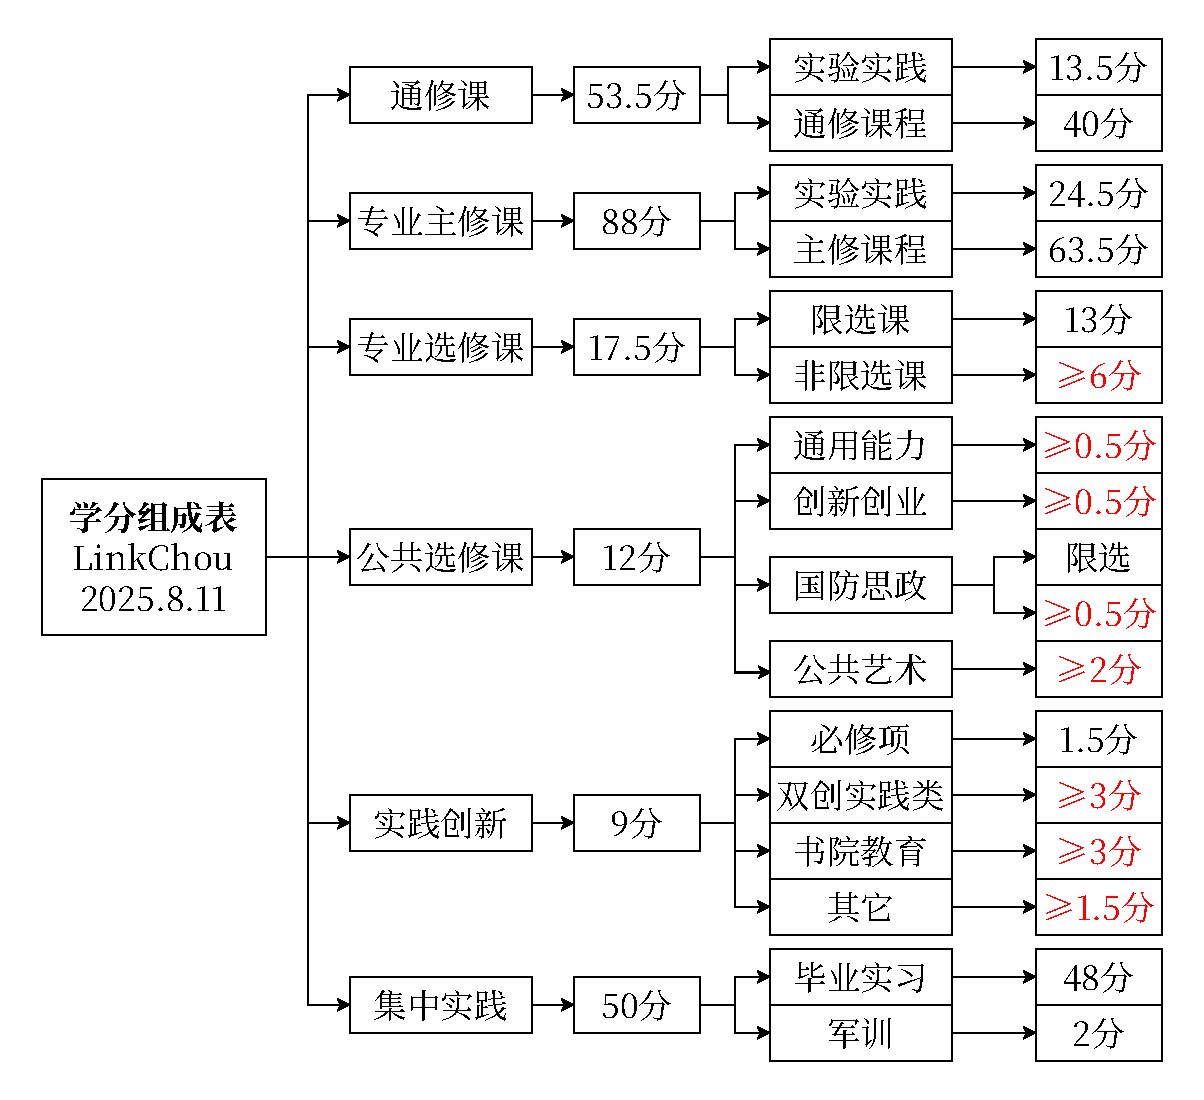
\includegraphics[width=\textwidth]{resources/sundry/学分.pdf}
    \label{score}
\end{table}

\newpage

\section[关于选修课的补充说明]{关于选修课的补充说明}
\begin{enumerate}
    \item 选修课分专业选修和公共选修两大类(详见\uline{\ref{score}}),\textbf{推荐在大一全年、大二上学期就把各类选修学分全都修满},这样就不用在后面学业愈重的情况下兼顾选修课的学习了,可以专心针对专业课程进行深入学习
    \item 专业选修课有限选和非限选之分,限选的课程无需操心,教务系统会自动选课,只需要保证非限选的课程学分达标即可
    \item 公共选修课每一类都要选至少一门,且需要满足总分,其中部分类别还有额外要求(详见\uline{\ref{score}}),国防教育类有国家限选课程(到时候看具体通知,会说的很明白的)
    \item 公共选修课有一部分是在教室上的,还有一部分是线上课程(使用“知到”app进行学习,大多数有平时分,不能突击),可以根据自己的实际情况选择\footnotemark
          \footnotetext{一般来讲线下课好过,每星期去一次教室听听课就行,结课考试也很简单;但是线上课随时都能刷课,刷完课考完试就不用每周都去听课了,根据自己的需求选择。}
    \item \textbf{\uuline{公共选修课联盟的公共选修课程不算学分、不收学费}}
\end{enumerate}

\section[自习禁止事项]{自习禁止事项}
\begin{enumerate}
    \item \textbf{禁止在教室内亲嘴、喧哗、频繁说话}
    \item \textbf{禁止在自习室内抖腿}
    \item 禁止外放音乐、视频等
    \item 禁止在大服、非本班上课常用教室占座
    \item 禁止在教室内食用气味浓的食物(例如榴梿、辣条等)
    \item 禁止长时间占用教室内电源插座,仅允许应急充电
    \item 禁止在教室以及教室旁厕所内吸烟
\end{enumerate}

\section[其他说明]{其他说明}
\begin{enumerate}
    \item \textbf{有以下情况将无法获得学位证:}
          \begin{enumerate}
              \item 修不够每项对应的学分
              \item 受过记过及以上处分
              \item 考试不合格累计补考课程每学年平均>5学分,且平均学分绩点<2.0
              \item 其他不符合相关要求的情况
          \end{enumerate}
    \item \textbf{大一不参与四六级,大二才能报名四六级考试}
    \item \textbf{\uuline{转专业}\footnotemark:}
          \footnotetext{依据教务处2024年5月21日发布的\uline{\href{https://jwch.sdsmu.edu.cn/2024/0521/c2593a131550/page.htm}{《山东第二医科大学2024年普通全日制本科学生转专业工作方案》}}简化,具体规定详见链接。该规定每年不一,如有变动,以教务处政策为准。}
          \begin{enumerate}
              \item 需满足以下条件:
                    \begin{enumerate}
                        \item 取得学籍的普通全日制一年级本科在校生
                        \item 未受处分、思想过硬、符合体检要求
                        \item 第一学年必修课和专业限定选修课平均成绩在本专业排名前30\%,且未挂科
                        \item 公费医学生、春季高考、第二学士学位、贯通培养学生等以特殊招生形式录取的学生,国家有相关规定或者录取前与学校有明确约定的,不得申请转专业
                    \end{enumerate}
              \item 考试科目:思政、英语\footnotemark、数学,比例为1:1:1,考试时间150分钟,总分为150分
                    \footnotetext{高考小语种考生可选择小语种替代英语,需在报名时备注,不备注者参加英语考试。}
              \item 流程:
                    \begin{enumerate}
                        \item 核算学生第一学年学习成绩并公示各类数据
                        \item 8月31日开始报名
                        \item 9月5日组织考试(地点详见相关通知)
                        \item 9月6日~10日公示录取名单\footnotemark
                              \footnotetext{按照“分数优先,遵循志愿”的原则进行录取。}
                        \item 9月11日~12日报到
                    \end{enumerate}
          \end{enumerate}
    \item 关于奖学金\footnotemark:本校有国家奖学金、校长奖学金、校级3等级奖学金等
          \footnotetext{请注意,目前学校仅能通过本人身份开通的、已开户的、账户已激活的、无异常的工商银行储蓄卡发放奖学金,详情政策可咨询学校财务处。}
    \item 新生开学考试\footnotemark 的内容为高中英语、高中数学,旨在让各位同学收心
          \footnotetext{按照往年惯例,不公布具体成绩。}
    \item \textbf{关于档案填写:}入档资料具有不能涂改、不能标记、不能修正的特性,因此严禁使用修正液或修正带对其涂改(涂改修正后立即作废)。填表时务必确保各类时间填写正确、与原始档案一致。此外,建议初次填写时使用铅笔轻轻填写,待负责人确认无误后方可擦除后使用黑色中性笔或中油笔填写(入档纸张为特殊A4纸,厚、重、滑,难以自行复印)
    \item 挂科与补考、重修:各年级、院系要求不一,详见学校下发的学生手册及院系通知
    \item 关于实验课与实验服:在实验课上课时务必按要求正确洗手并佩戴头套、口罩、手套,着实验服,\textbf{\uuline{严禁任何人在任何其它地点(尤其是餐厅)着实验服}!}因在实验室中需频繁接触实验动物、微生物,\textbf{极其推荐将实验课书包与普通课书包分开}!
          \label{schoolbag}
\end{enumerate}

\section[早操与晚自习]{早操与晚自习}
\begin{enumerate}
    \item 早操时间一般为6:00~7:00,晚自习时间通常为19:00~21:00,教室22:00关闭
    \item 早操与晚自习贯穿整个大一\footnotemark,并且跑操与晚自习均有院系学生会不定时进行抽查出勤率等指标,最终结果计入班级综测(详见下文\uline{\ref{class_evaluation}})的评分
          \footnotetext{按照惯例,麻醉专业无早操,只需要大一、大二早晨七点签到。}
\end{enumerate}

\section[班级综测]{班级综测}
\label{class_evaluation}
\begin{enumerate}
    \item 班级综测是用于考核各班表现的评判指标和分配见习点的依据\footnotemark,每学期计算一次,截至见习
          \footnotetext{以截至见习之前的各学期平均班级综测成绩计算班级排名,公费班级根据本年级政策进行。}
    \item 由班级平均成绩、比赛类、表彰类等类别构成,详见学生手册(各年级要求不一)
    \item 班级综测直接决定本班级同学后期学习和生活所在的医院规模、等级和生活条件(例如宿舍有无空调、暖气、洗衣机,是否提供插座,是否有早操和晚查寝\footnotemark 等),请大家务必重视
          \footnotetext{这意味着能否在外租房居住。}
\end{enumerate}

\section[???]{???}

大一的基础课程是临床的根基,没有基础则空中楼阁。

\subsection[三阶段考试]{三阶段考试}
???
\subsubsection[一阶段考试]{一阶段考试}
???
\subsubsection[二阶段考试]{二阶段考试}
???
\subsubsection[三阶段考试]{三阶段考试}
???
\subsection[考研]{考研}
???
\subsection[执业医师考试]{执业医师考试}
???%学习方面
% 就业指引
\chapter[就业指引]{就业指引\footnotemark}
\footnotetext{特别感谢:本章节内容由临床医学院党委提供。}

\section[总述]{总述}
\subsection[就业形式]{就业形式}
\begin{enumerate}
    \item 毕业生趋势:数量逐年增多
    \item 考研趋势:考研人数保持高位报考,“逆向考验”增多,再“考研”现象多见
    \item 就业情况:高质量充分就业难度增大,考研、考公、考编是学生心目中的“高质量就业”
\end{enumerate}

\subsection[就业政策]{就业政策}
以山东省潍坊市为例,每个地市都有相应的政策,如就业补贴、创业补贴、人才补贴、安家补贴等人才政策。(可从人社部网站查找)
\bigbreak
部分常用政策及相关网站链接见下:
\begin{enumerate}
    \item 山东省人力资源与社会保障厅\uhref{http://hrss.shandong.gov.cn/articles/ch00300/202404/9dfeed90-6eb1-41dc-9ab3-a0fcedef8491.shtml}{《山东省级重点人才政策清单》}
    \item 潍坊市人力资源与社会保障局\uhref{http://rsj.weifang.gov.cn/zcfg/rszc/rczc}{《潍坊市人才政策》}(含人才引进政策、人才创业政策、人才就业政策、职称评审政策、人才激励政策等)
    \item 山东省人力资源与社会保障厅\uhref{http://103.239.153.109/sdjyweb/index.action}{山东公共就业人才服务网上服务大厅}
    \item \uhref{https://m12333.cn/weifang.aspx}{潍坊人社通}
\end{enumerate}

\section[常见就业形式]{常见就业形式}
\subsection[升学录取(含出国境)]{升学录取(含出国境)}
\subsubsection[考研]{考研}
考研是应届生的首选,如已经考过,要积极地从其他渠道进行就业。

以近年考验情况为参考,每届毕业生的过线率在70\%左右,当年最终录取50\%;“二战”、“三战”后的总体录取比例达70\%左右,与当年的过线率基本一致。即,有30\%左右的同学,最终是需要就业的。

请同学们根据自己的实际情况做好定位、统筹谋划、积极就业(可在备考同时考规培、助研助管等,一用一备,二战上岸或是二战失利仍有工作)

\subsubsection[第二学士学位]{第二学士学位}
适合于想成为复合型人才,需要有一个学校学习氛围的同学。可以以在校生的身份享有学校的学习资源和学习氛围;本校目前支持药学专业,其他学校还有很多

\subsection[住院医师规范化培训社会化招生(社会化规培)]{住院医师规范化培训社会化招生(社会化规培)}
是医学生就业升学的第二渠道,有以下一些优点:
\begin{enumerate}
    \item “两个同等对待”,相当于研究生毕业,入院招聘、职称晋升均同等对待
    \item “同工同酬”,规培期间社会化规培医生基本相当于医院的住院医师
    \item 计算工龄,且在医院积累三年工作经历,为后续就业积攒了优质工作经历和行业人脉资源,利于职业发展
    \item 规培是医学继续教育的一部分,职称晋升的必须,早规培早受益
    \item 规培期间考研不受影响,距离导师也近,可以“近水楼台先得月”
    \item 规培期间还可以申请在职硕士,三年后也有专硕学位
    \item 规培的政策、待遇还将继续优化,值得期待
    \item 研究生还有专陪
\end{enumerate}

\subsection[考公考编]{考公考编}
要积极获取信息、积极参与

有以下几种类型可供参考:
\begin{enumerate}
    \item 公务员如卫健委等
    \item 公立医院岗位
    \item 医学院校及职业院校教师、高校辅导员
    \item 国有企业(医药企业)等相关岗位
    \item 西部计划、三支一扶、乡村医生专项等政策性岗位
    \item 社区医院、乡镇医院等岗位
\end{enumerate}

\subsection[科研助理、管理助理]{科研助理、管理助理}
可以考取外校、科研院所、科研团队的科研助理、管理助理岗位,有不少可以“近水楼台先得月”,就近就便考研;还可以聘任医院、学校等的助研、助管岗位

\subsection[合同制、劳务派遣、第三方等到医院就业]{合同制、劳务派遣、第三方等到医院就业}
是曲线达成目标的方式,先选定就业单位、就业科室,然后在工作同时再考编制等,“先到先得”占住岗位。民营医院也是一个选择

\subsection[校医院等]{校医院等}
校医院,如大、中、小学的校医院、机场医生等

\subsection[医药企业、保险企业、健康查体企业等]{医药企业、保险企业、健康查体企业等}
临床也有很多毕业生进入企业,从事医药学术推广、医药代表、医学沟通顾问、医学信息专员、临床QC、医疗保险专员、健康专员等

\subsection[自由职业]{自由职业}
根据个人实际及兴趣爱好等实现其他形式就业,如自由职业、灵活就业等;直播带货、网文作家、网店店主等

\section[部分就业岗位信息链接]{部分就业岗位信息链接\footnotemark}
\footnotetext{部分链接为外部网站所整理,本处仅作汇总整理。敬请自行甄别筛选,谨防诈骗。}
\begin{enumerate}
    \item \uhref{https://www.ncss.cn}{国家大学生就业服务平台(24365校园招聘服务)}
    \item \uhref{https://job.ncss.cn}{教育部大学生就业网}
    \item \uhref{https://www.sdgxbys.cn}{山东高校毕业生就业信息网}(公众号“山东就业创业导航”)
    \item \uhref{https://www.sdbys.com}{就选山东・青年人才全链条服务平台}
    \item \uhref{https://wfmc.sdbys.com}{山东第二医科大学就业信息网}(公众号“山二医就业服务”)
    \item \uhref{https://www.med66.com/weishengdanweizhaopin/gonggao/wa2406033156.shtml}{正保医学教育网-2024年6月全国各级医疗卫生单位招聘公告汇总}
    \item 住院医师规范化培训(公众号“规培”、“规培基地”,小程序“规培宝”)
    \item 第二学士学位(公众号“第二学士学位”、“第二学士学位咨询台”,小程序“第二学士学位帮帮帮”)
    \item \uhref{http://job.mohrss.gov.cn}{中国公共招聘网}
    \item \uhref{https://www.newjobs.com.cn}{中国国家人才网}
    \item \uhref{https://www.yimaitongdao.com}{医脉同道}
    \item \uhref{https://www.jobonline.cn/probation/index}{就业在线-百万就业见习岗位募集}
\end{enumerate}%就业创业
%???与竞赛
%暂时停止编译
\chapter[???与竞赛]{???与竞赛}
\section[???]{???}
\subsection[社会实践]{社会实践}
\subsubsection[三下乡]{三下乡}
注:活动中使用的可以代表学校的图标如校徽等需要经过审核。
\subsubsection[青鸟计划(返家乡)]{青鸟计划(返家乡)}
\subsection[???]{???}
\subsubsection[文化艺术节]{文化艺术节}
\subsubsection[科技文化月]{科技文化月}
\subsubsection[百团纳新]{百团纳新}
\subsubsection[宿舍文化]{宿舍文化}
\section[竞赛]{???}
\subsection[大创]{大创}
\subsection[实践技能]{实践技能}
\subsection[泰山杯]{泰山杯}
\subsection[组胚]{组胚}

%???与竞赛

% 通用指南目录

\chapter[通用教程与常用信息汇总]{通用教程与信息汇总}

% 教程
\section[常用教程]{常用教程}

\subsection*{特别说明}
\begin{enumerate}
    \item 本节中所有上标“㊕”的网址仅在连接校园网时可成功访问相关服务。
    \item \textbf{严禁使用QQ、微信直接打开本文提及的一切网址,必须使用正常更新的主流浏览器打开!}
\end{enumerate}

\subsection[新生信息查询]{\uuline{新生信息查询}}
\label{freshman_query}
\begin{enumerate}
    \item 关注“山东第二医科大学学生之家”公众号
    \item 点击菜单栏中的“新生报到”→使用身份证号、手机号、验证码登录
    \item →根据其中的相关指引完成预报到流程
    \item →查看宿舍号、学号、班级、院系等相关信息,并根据个人需求选择是否订购军训套装、被褥套装\footnotemark 等
          \footnotetext{也可来校当场订购,详见系统及录取通知书说明。}
\end{enumerate}

\subsection[校园网]{校园网}
\subsubsection[无线连接]{无线连接}
\label{wifi_register}
\begin{enumerate}
    \item 激活:到校报到完成后,学校将按照个人身份证号在\uline{\href{http://210.44.80.65}{http://210.44.80.65}$^㊕$}为大家开通校园网账号,并告知初始密码\footnotemark,请按照下发的说明登陆并确认激活
    \item 在设置页面连接“sdsmu-net”并在上述页面输入密码即可使用
          \footnotetext{每年初始密码不同,详见班级群内具体通知。}
    \item \textbf{充值}:点击\uline{\href{https://slzfw.sdsmu.edu.cn:8800/home}{https://slzfw.sdsmu.edu.cn:8800/home}$^㊕$},并登录;或在校园网的登陆页面点击“自助服务”按钮\footnotemark,登陆后即可使用支付宝充值(微信支付暂时无法使用)
          \footnotetext{若点击按钮后网页显示“403 Error”,请将网址前缀“http”改为“https”,按回车即可。}
    \item 校园网流量当前政策为每月免费60G,超出部分按0.5¥/G收费
\end{enumerate}

\subsubsection[有线连接]{有线连接}
\begin{enumerate}
    \item 按照\uline{\ref{wifi_register}} 的教程激活校园网
    \item 将网线插入宿舍内的“H3C”盒子的底部右侧的接口内并正确连接到电脑\footnotemark
          \footnotetext{若始终无法连接,应检查网线的内部线排列顺序,从左到右应为“白橙橙,白绿蓝,白蓝绿,白棕棕”。}
          \begin{enumerate}
              \item 首次连接:
                    \begin{enumerate}
                        \item 打开“设置”→“网络和Internet”→“拨号”→“设置新连接”
                        \item →“连接到Internet”→点击“否,创建新连接(C)”→选择“宽带(PPPoE)(R)”
                        \item →输入自己的校园网帐号以及密码→勾选“记住密码”
                    \end{enumerate}
              \item 再次连接:
                    \begin{enumerate}
                        \item 打开“设置”→“网络和Internet”→“拨号”
                        \item →选中之前设置的网络→连接即可
                    \end{enumerate}
          \end{enumerate}
    \item  注:上述均为Win10/Win11教程,Mac教程暂无。
\end{enumerate}

\subsection[校园手机卡]{校园手机卡}
\begin{enumerate}
    \item \textbf{开通与否全凭自愿,是否开通校园卡不影响校园网的使用。}随录取通知书一并寄出。如遇强制开通可告知带班学长或自行反馈
    \item 通常内含至少100分钟全国通话、80G校园流量(仅山东省内所有高校可用)\footnotemark
          \footnotetext{详情优惠政策可咨询营业厅,如追求更多流量建议学校各账号不绑定校园手机卡,每年根据新优惠政策调整手机卡(需及时注意注销旧手机卡以防欠费导致的信用记录问题)。}
    \item 开学报到当天可前往大服,免费领取礼品
\end{enumerate}

\subsection[空调使用教程]{空调使用教程}
\label{air_control}
\begin{enumerate}
    \item 微信关注“海享租”公众号,点击公众号菜单“在线租赁”,并注册、登录
    \item 点击“扫一扫”→扫描空调右下角二维码进行租赁\footnotemark
          \footnotetext{若提示租赁失败,请按照软件提示联系同宿舍的学长/学姐退租,也可咨询学长学姐或向宿管反馈。}
    \item →租赁完成后,点击“设备”→“空调图标”→“时长”,进行充值
    \item →点击“设备”→“空调图标”→“成员管理”,在此页面下将宿舍全部成员权限设置为均可管理空调开关即可
    \item \textbf{注意:}空调使用时长收费(0.55元/小时),具体收费及租赁政策详见“海享租”公众号
\end{enumerate}

\subsection[浴室预约与使用]{浴室预约与使用}
\subsubsection[浮烟山校区]{浮烟山校区}
\label{shower_software_f}
\begin{enumerate}
    \item 软件基础设置:
          \begin{enumerate}
              \item 在手机应用市场下载“大白U帮”app
              \item 按照实际住宿情况注册
              \item 授予并开启“定位”与“蓝牙”权限
          \end{enumerate}
    \item 本楼层小浴室使用:
          \begin{enumerate}
              \item 带好洗浴物品前往公共厕所旁边的浴室排队
              \item 进入浴室,点击如右图所示的按钮(\noindent\mbox{
\includegraphics[height=2.4ex]{resources/sundry/bath.pdf}})→选择“蓝牙设备”→“点击进行时”
              \item →“洗澡”→“搜索洗澡”\footnotemark
                    \footnotetext{搜索不到设备请务必开启“蓝牙”功能,学校的设备无法扫码连接。}
              \item →选择设备\footnotemark →“开始洗澡”
                    \footnotetext{距离厕所入口最近的是1号,远的是2号;不确定可以询问学长。}
              \item 结束后点击“结束洗澡”按钮,并结算
          \end{enumerate}
    \item 一层公共大浴室预约:
          \begin{enumerate}
              \item 在软件初始界面根据实际情况选择“X号楼1层”的浴室
              \item →点击一个浴位,并点击“预约”按钮(若已满请选择“排队”)
              \item →在8分钟内前往浴室,并点击“开始洗浴”
              \item →结束后点击“结束洗澡”按钮,并结算
          \end{enumerate}
    \item 费用:以程序显示为准,详情收费标准略
    \item 申诉:如果在洗澡时突然停电导致无法结束洗澡而被扣费,请按照软件打开时弹出的公告,联系相关工作人员处理
\end{enumerate}
\subsubsection[虞河校区]{虞河校区}
\label{shower_software_y}
\begin{enumerate}
    \item 支付宝搜索“住理生活”小程序,并按照提示开通账户(建议支付宝绑定银行卡)
    \item →搜索“潍坊医学院虞河校区”,并绑定账号到自己性别的浴室
    \item →扫描设备二维码即可使用淋浴
    \item 也可在小程序主页面点击“洗浴”→“切换设备”→手动选择设备进行洗浴
    \item \textbf{注意:浴室营业时间为10:00~21:45,22:00停水,浴室位置较少,请错峰洗澡!}
\end{enumerate}
\subsubsection*{注意事项}
\begin{enumerate}
    \item 如果未点击“结束洗澡”按钮便直接离开可能会被多扣费
    \item 严令禁止在浴室内大便!!!
\end{enumerate}

\subsection[洗衣机/洗鞋机使用教程]{洗衣机/洗鞋机使用教程}
\subsubsection[浮烟山校区]{浮烟山校区}
\label{washing_machine_f}
\begin{enumerate}
    \item 在微信小程序搜索“海乐生活”,并注册、开启相机与定位权限
    \item 预约方法(也可直接使用):
          \begin{enumerate}
              \item 在小程序内点击“附近营业点”→找到“潍坊医学院X号楼”
              \item →选择相应的楼层→选中洗衣机并下单→等待上次洗衣结束
              \item →前往洗衣机→输入验证码→放入衣物与洗衣粉/洗衣液并缴费
          \end{enumerate}
    \item 扫码直接使用(不可预约):
          \begin{enumerate}
              \item 前往洗衣机→在小程序内点击“扫码使用”按钮
              \item →扫描洗衣机上的二维码→选择并下单
              \item →放入衣物与洗衣粉/洗衣液,输入验证码后缴费即可
          \end{enumerate}
    \item 收费标准详见软件说明
    \item 洗衣机错误处理办法(若无相关经验切忌自行操作):
          \begin{enumerate}
              \item 拨打洗衣机旁边的报修电话;
              \item E1:洗衣机断电后开门,打开洗衣机右下角小门,旋开阀门,使用镊子等工具伸入并清除其中堵塞管道的杂物,恢复原样即可;
              \item E4:旋开洗衣机后方的水管阀门即可。
          \end{enumerate}
\end{enumerate}
\subsubsection[虞河校区]{虞河校区}
\label{washing_machine_y}
\begin{enumerate}
    \item 微信小程序搜索“智慧笑联”→按照提示注册并授予定位权限
    \item →绑定“潍坊医学院(虞河校区)”→绑定至自己所在的宿舍楼
    \item →再次扫描洗衣机上的二维码,按提示操作并付款即可
    \item 收费标准详见软件说明
\end{enumerate}

\subsubsection[禁止事项]{禁止事项}
\begin{enumerate}
    \item 禁止向第二格内倾倒洗衣粉、洗衣液,\textbf{第二格是放柔顺剂的}!
    \item \textbf{禁止使用洗衣机洗鞋},请用旁边的洗鞋机!
    \item 禁止在洗衣机上堆放杂物
    \item \textbf{\uuline{禁止将袜子、内衣内裤等贴身衣物机洗!}}
\end{enumerate}

\subsection[烘干机使用教程]{烘干机使用教程}
\label{dry_machine}
\begin{enumerate}
    \item 注册等步骤详见\uline{\ref{washing_machine_f}}
    \item 按照预约的方法,选择宿舍楼后,选择“烘干机”即可,其他步骤与洗衣相似
    \item 推荐烘干配置
          \begin{enumerate}
              \item 高温60分钟:大部分轻薄的衣物(例如T恤、卫衣、浴巾等)
              \item 高温120分钟:薄被(如夏凉被)
          \end{enumerate}
    \item \textbf{注意:}\textbf{使用前后务必控干水箱并清理滤网。}棉被、羽绒服等禁止使用烘干机烘干以免损坏及不必要的危险情况发生。
    \item 收费标准详见软件提示
\end{enumerate}

\subsection[吹风机使用教程]{吹风机使用教程}
\label{hair_drier}
\begin{enumerate}
    \item 每层公共浴室旁边有两个公用吹风机,需扫码\footnotemark 租赁使用
          \footnotetext{部分吹风机屏幕二维码可能有缺损,不易扫描成功,多次尝试即可。(推荐使用浏览器扫码并复制到微信内收藏该网址,下次直接在微信内点击即可使用。)}
    \item →待手机发出“滴--滴”的声音后租赁成功
    \item →将手机扬声器对准吹风机租赁器方可正常使用
    \item 收费标准:详见软件提示,1分钱起步
\end{enumerate}

\subsection[图书馆座位预约教程]{图书馆座位预约教程}
\label{library_book}
\begin{enumerate}
    \item 微信小程序搜索“青栀校园”→微信注册登录并绑定学号→允许小程序通知
    \item →在小程序内点击“座位预约”或扫描图书馆座位上的二维码即可
    \item \textbf{座位暂离的注意事项:}
          \begin{enumerate}
              \item 如因各种原因需要长时间离开的,请在小程序上选择“暂时离开”,否则按违规处理
              \item 离馆时也需要在小程序内确认
              \item 如发现已预约的座位被他人占据,请扫描桌面上的二维码并在小程序内举报,工作人员将尽快处理
          \end{enumerate}
    \item \textbf{违规说明:}
          \begin{enumerate}
              \item 已预约而未按时到位的记一次违规
              \item 未选择暂离而离开座位被举报的记一次违规
              \item 停止使用后未选择退馆的记一次违规
              \item \textbf{三次违规后将取消座位预约资格三天}
          \end{enumerate}
    \item 其他禁止事项
          \begin{enumerate}
              \item 禁止占用其他人已经预约的座位
              \item 禁止在图书馆内喧哗、吸烟
              \item 禁止在图书馆的非背诵区域内背诵、朗诵、频繁交流
              \item 禁止在图书馆内谈恋爱、亲嘴
          \end{enumerate}
\end{enumerate}

\subsection[设施报修方式枚举]{设施报修方式枚举}
\label{repair_report}
\begin{enumerate}
    \item 宿舍维修(浮烟山校区):
          \begin{enumerate}
              \item 加入各宿舍楼的QQ报修群,在群内反映具体故障
              \item 前往一层宿管处填表报修
              \item 在宿舍一层宿管旁边的公告栏处查看相关负责人的电话,直接拨打即可
              \item 拨打学生公寓管理中心电话反馈
              \item 询问带班学长、学姐
          \end{enumerate}
    \item 教室维修(浮烟山校区):
          \begin{enumerate}
              \item 拨打后勤管理处的电话报修
              \item 拨打教室管理中心的电话报修(仅限多媒体及饮水机)
              \item 拨打物业电话报修
              \item 在“诉求留言”微信小程序内反馈
          \end{enumerate}
    \item 宿舍维修(虞河校区):在宿管处填写报修单据并送往物业维修中心(位置见此\uline{\ref{common_locations_yuhe}})
    \item 教室维修(虞河校区):拨打教室内张贴的报修电话
\end{enumerate}

\subsection[缓考申请教程]{缓考申请教程\footnotemark}
\footnotetext{各学院要求不一:临床医学院大部分课程可以只填写钉钉、教务系统,仅少数要求同时提交纸质表格;其他学院以教师要求为准。}
\begin{enumerate}
    \item 填写钉钉\footnotemark(详细步骤如下)
          \footnotetext{需在学校统一将大家拉入钉钉的“山东第二医科大学”企业后方可使用。}
          \begin{enumerate}
              \item 打开钉钉→点击左上角选择主企业为“山东第二医科大学”
              \item →点击页面最下方菜单栏“工作台”→点击“OA审批”
              \item →在“学风建设”类选择“学生缓考审批表”(或直接搜索“学生缓考审批表”)
          \end{enumerate}
    \item 在教务处下载《\uline{\href{https://jwch.sdsmu.edu.cn/_upload/article/files/f7/d0/c172c4f74eecba307f700cde1a21/99599310-0254-48be-adc5-fcafa99e7341.doc}{山东第二医科大学学生缓考审批表}}》,打印3份并按照要求填写完毕
    \item 填写教务系统(详细步骤如下)
          \begin{enumerate}
              \item 进入教务系统(仅校园网,详情参见\uline{\ref{academic_affairs_system}})
              \item 点击左侧菜单“考试报名”→“我的申请”→“缓考申请”
              \item →选择“学年学期”和“活动名称”后,直接点击“搜索”(不要填写科目名称)
              \item →在弹出的菜单中选择缓考科目并填写申请\footnotemark
                    \footnotetext{若因病缓考体测,需要上传病历本等相关材料,并前往校医院开具证明,再前往学工办向教师当面说明情况。}
          \end{enumerate}
    \item 前往学工办交表并等待审批
\end{enumerate}

\subsection[多媒体教室申请流程]{多媒体教室申请流程}
\begin{enumerate}
    \item 打印《\uline{\href{https://xshch.sdsmu.edu.cn/_upload/article/90/9a/94414f104377acc23eee081ca976/e714b474-f0af-4f44-b081-a5bfff20e393.doc}{多媒体教室使用审批表}}》并填写
    \item 前往本年级学工办签字、盖章
    \item 前往教室E区2层(见\uline{\ref{map_fuyanshan_teach_building}})靠近A区处的“教室管理中心”签字盖章
    \item 前往预约的教室,拨打讲台上教室管理员的电话提前沟通说明
\end{enumerate}

\subsection[乐道济世书院教室申请流程]{乐道济世书院教室申请流程}
\begin{enumerate}
    \item 打印《\uline{\href{https://xshch.sdsmu.edu.cn/_upload/article/files/1f/59/48196a87425186f3db9eb6fbd219/cdbf8cf8-d42a-4dd3-894d-5fb5df83ee13.doc}{乐道济世书院入驻申请表}}》并填写
    \item 前往本年级学工办签字、盖章
    \item 前往书院西侧的“书院管理办公室”签字盖章(书院位置见\uline{\ref{map_fuyanshan_holistic}})
\end{enumerate}

\subsection[学生会校级格式]{学生会校级格式}
\begin{enumerate}
    \item 用途:校级格式是一种用于校内各类\textbf{正式文稿}(如活动通知、综测条例、学生会文件等)的标准
    \item 具体要求:
          \begin{enumerate}
              \item 纸张大小:A4纸
              \item 装订:页面左侧上下各 $\frac{1}{4}$ 处,距左边界0.3--0.5㎝处,钉与纸张左边界平行
              \item 页边距:上下左右均为2.5㎝
              \item 页码:两页及以上的材料,在页面底端居中插入
              \item 行间距:固定值,26磅
              \item 标点:均为中文标点,除特殊情况\footnotemark 外不应使用英文标点
                    \footnotetext{特殊情况举例:时间(22:05),英文活动(So, let us practice English!)等。}
              \item 文章标题格式:方正小标宋简体,小二号,居中
              \item 标题与正文之间空一行
              \item 正文格式:仿宋-GB2312,三号,两端对齐,首行缩进2字符
              \item 正文一级标题格式:“\textbf{一、}”;黑体,三号,居左,首行缩进2字符
              \item 正文二级标题格式:“\textbf{(一)、}”;楷体-GB2312,三号,居左,首行缩进2字符
              \item 正文三级标题格式:“\textbf{1、}”;其他要求与正文相同
              \item 正文四级标题格式:“\textbf{(1)}”;其他要求与正文相同
              \item 正文与落款之间空2行
              \item 落款机构(个人姓名)格式:仿宋-GB2312,三号,右对齐
              \item 落款时间格式:仿宋-GB2312,三号,右对齐,时间格式范例:2024年02月10日
          \end{enumerate}
\end{enumerate}

\subsection[小组汇报PPT制作指南(初级)]{小组汇报PPT制作指南(初级)}
\begin{enumerate}
    \item 整体要求
          \begin{enumerate}
              \item 选择软件:请使用大多数人使用的微软\ Office办公软件,或者金山WPS最新版;并在电脑上进行编辑,手机当且仅当用于ppt的简单查看。如无特殊情况不要使用LibreOffice、OpenOffice、腾讯文档等办公套件以免不兼容。
              \item \textbf{明确比例}:PPT(也称Slide)有4:3与16:9两种主流比例\footnotemark
                    \footnotetext{注:4:3比例像正方形,16:9是明显的长方形;下述的各类参数(如:24/32号字体)均以4:3、16:9的顺序进行。}
              \item 首页规范:首页应含有所有的必要信息(详情见下文)
              \item 目录规范:PPT应当在第二页含有一个简洁明了的目录
              \item 内容规范:\textbf{PPT内仅应含有所讲内容的关键部分}而非一昧照抄原文
              \item 字体与段落规范:\textbf{PPT字体不应过小,间距不应过密}(详情建议见下文);禁止使用文字阴影;\textbf{特殊字体必须内嵌于PPT}(例如艺术字、书法体等),禁止现场在演示的电脑上下载补全需要的字体(操作步骤可搜索“在PPT内嵌入字体”)
              \item 图片规范:每张图片不应大于10M\footnotemark,如发现图片模糊,需手动检查PPT设置,将PPT更改为“禁止自动压缩图片”,操作步骤请自行搜索
                    \footnotetext{如果图片过大,可以使用\uline{\href{https://gitee.com/LinkChou/rimage_gui/releases/latest}{Rimage\_GUI}}适当缩小图片体积(软件开源,如被报毒请自行分辨)。}
              \item 动画规范:\textbf{PPT不应有过多动画以及元素堆叠}(例如,绝对禁止PPT中的一页内含15张大图片,依靠动画一张张切换,以免软件突然崩溃)
              \item 配色规范:请\textbf{使用经典的“文字—背景”配色}(\sout{虽然确实难看}),例如“黑—白”,“红—白”,\linebreak[3]“白—黑”,“蓝—白”等,切勿使用“橙—白”、“红—蓝”等投影后效果一塌糊涂的配色\footnotemark
                    \footnotetext{请注意ppt配色以使色觉感知局限的同学能顺畅接受信息。}
              \item 文件命名规范:要求PPT文件名\textbf{简单易懂,包含所有必须信息}
              \item 文件保存规范\footnotemark:\textbf{必须同时以“.pptx”后缀与“.ppt”后缀各保存一份}以免部分电脑无法正常打开,\textbf{禁止保存为“.dps”、“.odp”等特殊格式},详情见下
                    \footnotetext{\textbf{若无法看到文件名称后缀,请搜索“电脑设置显示文件扩展名”。}}
              \item 学校校徽及图标等标识使用规范:详情见\uline{\href{https://www.sdsmu.edu.cn/4229/list.htm}{《山东第二医科大学VIS视觉识别系统手册》}}(由校宣传部印发)
          \end{enumerate}
    \item 详细要求:
          \begin{enumerate}
              \item 首页:需注明小组成员姓名及学号,日期,课程名称,授课教师等必要信息并\textbf{仔细检查是否有误},标题的字体不应小于80/75号,小组成员及其他信息字体不应小于25/25号
              \item 目录页:简短凝练,总字数不应超过35个字;字体不应小于80/55号
              \item 内容页:字体\footnotemark 不应小于55/40号,上下左右应各留出 $\frac{1}{10}$ 左右的间距;如内容过多应自行分页,\textbf{严禁为节省页数而缩小字号};PPT显示的内容与口述补充的内容在6:4或7:3左右最佳,各类关键数据的引用(例如学术数据、课标外的公式定义等)应当按照\linebreak[3]《\textbf{GB/T}\ 7714—2015 信息与文献 参考文献著录规则》的相关标准\textbf{标明出处}
                    \footnotetext{下面的字体皆以微软雅黑为标准,楷体、仿宋等纤细字体请自行增加字号。}
              \item 文件命名\footnotemark:推荐使用“\textbf{20XX级临床X班X组关于XXX的汇报(终稿).pptx}”此类命名,\textbf{严禁使用默认名称以防混淆}(例如“新建 Microsoft PowerPoint 演示文稿.pptx”)。此外,在ppt未定稿时,推荐使用一些默认的规范进行命名(例如“\textbf{关于XXX的汇报草稿-4.pptx}”),以方便小组成员确定PPT版本,而非使用默认的“新建 Microsoft PowerPoint 演示文稿(1)(2)(5).pptx”这种高血压命名。
                    \footnotetext{文件名称后缀的“.pptx”、“.ppt”等各种类型并非手动添加,而是文件自带,\textbf{严禁手动修改后缀名!}}
              \item 文件保存\footnotemark:如需在“.ppt”“.pptx”两种格式间相互转换请使用PowerPoint或WPS等办公软件,“.dps”格式必须使用WPS才能转换为“.ppt”或“.pptx”格式。
                    \footnotetext{\textbf{转换方法}:在左上角的“文件”菜单选择“另存为”,在下拉框中选择“.pptx”并保存。}
          \end{enumerate}

\end{enumerate}

\subsection[钉钉请假流程]{钉钉请假\footnotemark 流程}
\label{leave_dingtalk}
\footnotetext{需在学校统一将大家拉入钉钉的“山东第二医科大学”企业后方可使用。\textbf{各学院要求不一,仅以临床医学院为例。}}
\begin{enumerate}
    \item 线下请假步骤(正常情况):
          \begin{enumerate}
              \item 前往学工办或班主任办公室,当面请假并获得假条
              \item →根据老师要求扫描相关二维码→钉钉填表
              \item →刷脸进出校门,并将请假条之一交给保卫处
              \item →返校后,在钉钉的电子假条处,以评论的方式销假
          \end{enumerate}
    \item 线上请假步骤:
          \begin{enumerate}
              \item 打开钉钉→点击左上角选择主企业为“山东第二医科大学”
              \item →点击页面最下方菜单栏“工作台”→点击“OA审批”
              \item →在“学生日常事务管理”类选择“浮烟山校区本科学生请假单”→填表
              \item →电话联系班主任老师或学工办老师,说明请假事由并等待审批
              \item →审批通过后刷脸进出校门
              \item →返校后,在钉钉的电子假条处,自觉以评论的方式销假
          \end{enumerate}
          \textbf{注意:}请大家自觉销假,切忌一再拖延。
\end{enumerate}

\subsection[家长、校友进校参观指南]{家长、校友进校参观指南\footnotemark}
\footnotetext{注:本节仅适用浮烟山校区;虞河校区为开放校区,除宿舍、教学楼外,均可参观。}
\begin{enumerate}
    \item 学校在每年8月30日前后允许家长参观校园\footnotemark,具体政策以学校官方说明为准
          \footnotetext{允许社会车辆在参观时段在校园内划定的区域内停放,(通常)允许家长在规定时间内参观宿舍环境,具体政策每年不同,具体情况以学校官方说明为准。}
    \item 其他校友若有返校需求可凭本人毕业证、学生证等有效证件(电子版也可),或通过当年所在院系的老师联系保卫处,在校门口登记后即可入校参观
\end{enumerate}

\subsection[缴费教程]{缴费教程}
\label{fee_pay}
\begin{enumerate}
    \item 官方:微信公众号“山东第二医科大学财务处”或“\uline{\href{http://tyzfpt.sdsmu.edu.cn/xysf/login.aspx}{山东第二医科大学校园统一缴费平台}}”
    \item 用途:学费缴纳、卡号绑定等
    \item 学费缴纳教程:
          \begin{enumerate}
              \item 前往公众号菜单,点击右下角“缴费管理”→“支付平台”
              \item →登录系统(帐号为学号,初始密码为姓首字母大写加身份证后六位)
              \item →按照提示修改初始密码(请务必牢记)→进行缴费
          \end{enumerate}
    \item 银行卡绑定教程:
          \begin{enumerate}
              \item 目的:学校仅在初次使用时收集一次卡号并存储数据,以便下次直接使用\footnotemark
                    \footnotetext{详情见学校官方说明。}
              \item 打开“山东第二医科大学财务处”公众号,点击“财务中心”
              \item →使用帐号密码登录并绑定微信号(帐号为学号,初始密码为000000)
              \item →点击“卡号维护”→“管理”
              \item →按照提示填写相关信息,确认信息无误后提交即可
          \end{enumerate}
\end{enumerate}

\subsection[学工系统(微信小程序)]{学工系统(微信小程序)}
\begin{enumerate}
    \item 用途:学工系统主要用于晚点名、返校信息填报等日常工作\footnotemark
          \footnotetext{原“请假审批”、“外出审批”工作已基本转移至“钉钉”,教程参见\uline{\ref{leave_dingtalk}}。}
    \item 使用方式:
          \begin{enumerate}
              \item 打开“定位权限”并允许微信使用→在微信搜索“智慧学工”小程序
              \item 根据学校下发的账号密码进行登录(推荐立即与微信绑定以免忘记密码)
          \end{enumerate}
\end{enumerate}

\subsection[教务系统]{\textbf{\uuline{教务系统}}}
\label{academic_affairs_system}
\begin{enumerate}
    \item 官网:\uline{\href{https://jwgl.sdsmu.edu.cn}{https://jwgl.sdsmu.edu.cn}$^㊕$}
    \item 用途:\textbf{选课,缓考申请,成绩查询},查看(导出)课程表,空闲教室查询
    \item \textbf{注意:}仅限校内访问,如需在外使用教务系统,参见\uline{\ref{cas_system}}条目
\end{enumerate}

\subsection[CAS资源访问控制系统(校内VPN)]{\textbf{\uuline{CAS资源访问控制系统(校内VPN)}}\footnotemark}
\footnotetext{在校内时可通过校园网直接访问相应系统,无需使用本系统中转。}
\label{cas_system}
\begin{enumerate}
    \item 官网:\uline{\href{https://webvpn.sdsmu.edu.cn}{https://webvpn.sdsmu.edu.cn}}
    \item 说明:(也称CAS认证系统)本系统用于\textbf{在校外访问校内网络信息资源},如:教务系统(查成绩、课表)、知网、临床医学虚拟仿真实验中心\footnotemark 等
          \footnotetext{查阅文献推荐使用CARSI系统,速度快效果好,教程详见\uline{\ref{carsi_system}}。}
    \item 异地登录教务系统教程(其它系统同理):
          \begin{enumerate}
              \item 打开网站,点击“统一身份认证登录”,按照学校下发的专用账号、密码登录即可(推荐绑定微信)
              \item →找到应用中心→“教务系统—非单点登录”\footnotemark →使用教务系统账号密码登录即可
                    \footnotetext{请注意,在校外时点击“教务系统”无法登录,只有“非单点”能校外登录!}
          \end{enumerate}
\end{enumerate}

\subsection[CARSI系统]{\textbf{\uuline{CARSI系统}}}
\label{carsi_system}
\begin{enumerate}
    \item 官网:\uline{\href{https://ds.carsi.edu.cn}{https://ds.carsi.edu.cn}}
    \item 说明:(与CAS认证系统作用不同)用于快速访问学校订阅的各类数据库,如百度文库、知网、万方、维普等
    \item 使用教程:
          \begin{enumerate}
              \item 进入官网→搜索“山东第二医科大学”并勾选“记住我的选择”→点击后进入登陆界面\footnotemark
                    \footnotetext{请注意,不要收藏登录界面的网址!每次登录网址都不一样,只能从官网重新进入!}
              \item →使用\textbf{CAS认证系统}的账号密码登录系统,出现各类弹窗一律选择“Accept”即可\footnotemark
                    \footnotetext{仅推荐在自己的电脑上如此设置,如必须在网吧等公共场所的电脑上使用,请审慎阅读相关提示,并谨慎进行登录,如因账号泄露造成损失,一切责任自负。}
              \item →登录完成后,点击任意资源链接即可进入相应网站并获取论文
          \end{enumerate}
\end{enumerate}

\subsection[校务行(微信小程序)]{校务行(微信小程序)}
\label{cert_prover}
\begin{enumerate}
    \item 官网:微信小程序
    \item 用途:查成绩,下载学籍证明、成绩证明的pdf版本
    \item 费用:以程序显示为准
    \item 教程:
          \begin{enumerate}
              \item 搜索小程序“校务行”
              \item →点击右上角“点击登录”(帐号为学号,密码为身份证后六位)\footnotemark
                    \footnotetext{新生可能无法在开学后即刻使用本程序,需等待学校将信息录入完毕。}
              \item →按需选择“电子成绩单”或“电子证明”→按照小程序提示进行即可
          \end{enumerate}
\end{enumerate}

\subsection[档案查询]{档案查询}
\subsubsection[档案远程服务利用系统(学校)]{档案远程服务利用系统(学校)}
\begin{enumerate}
    \item 官网:\uline{\href{https://dangan.sdsmu.edu.cn/service-utilization/web/management/index}{https://dangan.sdsmu.edu.cn/service-utilization/web/management/index}}
    \item 微信公众号入口(与官网作用相同):“山东第二医科大学”公众号→微服务→档案查询
    \item 业务范围:
          \begin{enumerate}
              \item 招生录取名册(学生登记表)
              \item 学生成绩
              \item 其他学籍档案
              \item 查档预约、查档咨询
          \end{enumerate}
    \item 其他注意事项详见官网
\end{enumerate}
\subsubsection[高校档案查询利用平台]{高校档案查询利用平台}
\begin{enumerate}
    \item 官网:\uline{\href{http://gxda.dag.shandong.gov.cn:81/index}{http://gxda.dag.shandong.gov.cn:81/index}}
    \item 业务范围:同“档案远程服务利用系统”
\end{enumerate}

\subsection[心理健康教育中心预约教程]{心理健康教育中心预约教程}
\begin{enumerate}
    \item 作用:纾解心理压力、提供心理咨询等
    \item 工作时间(周一至周五):08:00~11:30、14:00~17:30
    \item 提示:预约后1个工作日左右,咨询中心将回电联系并协商心理咨询时间,请注意接听电话
    \item 线下预约:至浮烟山校区E206填表后等待咨询中心回电
    \item 电话预约:拨打0536-8462130
    \item 线上预约:填写\uline{\href{https://www.wjx.cn/vm/YOHd59S.aspx}{心理咨询信息登记表}}后等待回电

\end{enumerate}

\subsection[常见证明申请]{常见证明申请}
\begin{enumerate}
    \item 说明:适用于学籍证明\footnotemark、成绩证明
          \footnotetext{在考试时,学生证与学籍证明拥有相同效力,丢失学生证可使用学籍证明代替。}
    \item 线下打印
          \begin{enumerate}
              \item 携带身份证、手机前往D区的打印机,详情位置见此\uline{\ref{common_locations_fuyanshan}}
              \item 按照机器的说明填写相关信息并打印
              \item 无纸时请按照机器上的相关联系方式联系工作人员
          \end{enumerate}
    \item 线上下载
          \begin{enumerate}
              \item 按照\uline{\ref{cert_prover}}的教程申请并下载,自行前往打印店打印即可(请注意及时删除打印完毕的文件以免泄漏隐私)
          \end{enumerate}
\end{enumerate}

\subsection[监控录像调取等申请]{监控录像调取等申请}
\label{sdsmu_app}
\begin{enumerate}
    \item 用途:调取监控录像、申请课程录制等
    \item 按照 \uline{\ref{cas_system}} 处的说明登录“山东第二医科大学App”
    \item 点击下方菜单栏“应用”→“业务申请”
    \item 按需选择“保卫处调阅监控录像审批流程”等申请
\end{enumerate}

\subsection[公交信息与免费乘车指南]{公交信息与免费乘车指南}
\label{free_bus}
免费线路\footnotemark:9、13、19、29、63、69、71、101、109、166、167
\footnotetext{据《滨海及浮烟山两地大学城在校学生免费乘坐校区至中心城区公交车实施方案》(潍交城〔2024〕5号)内容,免费公交政策暂行时间为:2024.04.29~2025.04.28。在此期间持学生证即可免费乘车。}
\begin{tblr}[
        long,
        caption = {常用站点名称对应关系一览表},
    ]{
        cells = {c,m},
        rowhead = 1,
        row{1} = {cmd=\bfseries},
        vlines,
        hlines,
        cell{2,7,29,31}{1} = {r=2}{},
        cell{4,9,19,22}{1} = {r=3}{},
        cell{12}{1} = {r=4}{},
        cell{27,30}{3} = {r=2}{},
        hline{1-2,7,12,16,34} = {-}{1pt},
    }
    常见目的地       & 具体方位     & 站点名                   \\
    浮烟山校区       & 南门         & 山东第二医科大学南门     \\
                     & 北门         & 山东第二医科大学北门     \\
    虞河校区         & 北门         & 胜利街虞河路路口西       \\
                     & 东门         & 虞河路胜利街路口南       \\
                     & 北侧         & 鸢飞路胜利街路口北       \\
    附属医院         & 西南侧       & 附属医院                 \\
                     & 南侧         & 福寿街虞河路路口东       \\
    人民医院         & 本部东门     & 人民医院东门             \\
                     & 本部西侧     & 人民医院                 \\
                     & 北辰院区南门 & 北辰院区                 \\
    火车站           & 北广场       & 火车站                   \\
                     & 东侧         & 青年路铁路桥北           \\
                     & 东北侧       & 火车站                   \\
                     & 潍坊北站     & 高铁北站                 \\
    人民公园         & 西门         & 人民公园西门             \\
    市中医院         & 东门         & 市中医院                 \\
    妇幼保健院       & 东门         & 潍坊市妇幼保健院潍城院区 \\
    泰华城           & 北侧         & 泰华城                   \\*
                     & 西南侧       & 青年路胜利街路口南       \\*
                     & 南侧         & 风筝广场                 \\
    万达广场         & 西侧         & 鸢飞路福寿街路口南       \\
                     & 南侧         & 潍坊中学                 \\
                     & 北侧         & 福寿街鸢飞路路口东       \\
    谷德广场         & 南侧         & 谷德广场                 \\
    奎文防疫站       & 无           & 奎文防疫站               \\
    鲁台会展中心     & 北门         & 鲁台会展中心             \\
    蓝海大饭店       & 南门         &                          \\
    谷德锦           & 南侧         & 北宫街清平路路口西       \\
                     & 东侧         & 潍坊交通职业中等专业学校 \\
    奥林匹克体育公园 & 东侧         &                          \\
                     & 南侧         & 奥体中心                 \\
    十笏园           & 西侧         & 十笏园
\end{tblr}

\begin{tblr}[
        long,
        caption = {常用路线汇总表},
        note{1} = {加粗线路为上述免费乘车线路。},
    ]{
        rowhead = 1,
        cells = {c,m},
        row{1} = {cmd=\bfseries},
        cell{1}{2} = {c=3}{},
        cell{2,7,9,13,18,23}{1} = {r=2}{},
        cell{4}{1} = {r=3}{},
        cell{4,16,17,20,21,25}{1} = {}{cmd=\bfseries},
        vlines,
        hlines,
    }
    路线\TblrNote{1} & 常见目的地           &                          &                  \\
    5                & 火车站(北广场)     & 市中医院(东门)         & 风筝广场         \\
                     & 万达广场(西侧)     &                          &                  \\
    13               & 浮烟山校区(南门)   & 虞河校区(北门)         & 火车站(东侧)   \\
                     & 附院(西门)         & 泰华城(南侧)           & 妇幼保健院       \\
                     & 奎文防疫站           & 人民公园                 & 风筝广场         \\
    22               & 泰华城(北侧)       & 十笏园                   & 谷德锦           \\
                     & 奥林匹克公园         &                          &                  \\
    23               & 火车站(北广场)     & 附院(南侧)             & 十笏园           \\
                     & 万达广场(北侧)     &                          &                  \\
    D28              & 人民医院(本部东门) & 人民医院(北辰院区南门) &                  \\
    56               & 火车站(北广场)     & 泰华城(北侧)           & 谷德广场         \\
    59               & 虞河校区(北门)     & 虞河校区(东门)         & 人民医院(东门) \\*
                     & 谷德锦(南侧)       & 奥林匹克公园(东南侧)   &                  \\
    66               & 虞河校区(北门)     & 市中医院                 & 万达广场(南侧) \\
    69               & 浮烟山校区(北门)   & 火车站(东侧)           & 火车站(北广场) \\
    71               & 浮烟山校区(北门)   & 火车站(东侧)           & 火车站(北广场) \\
    75               & 虞河校区(北侧)     & 万达广场(西侧)         & 风筝广场         \\
                     & 火车站(北广场)     &                          &                  \\
    101              & 浮烟山校区(北门)   & 火车站(北广场)         &                  \\
    109              & 浮烟山校区(南门)   & 泰华城(东北侧)         &                  \\
    132              & 人民医院(本部西侧) & 万达广场(西侧)         &                  \\
    162              & 虞河校区(东门)     & 人民医院(东门)         & 附院(西门)     \\
                     & 奎文防疫站           &                          &                  \\
    167              & 浮烟山校区(南门)   & 鲁台会展中心(北门)     & 蓝海大饭店
\end{tblr}

\subsection[高铁学生票购买流程]{高铁学生票\footnotemark 购买流程}
\footnotetext{仍保留线下优惠资质核验、学生票购买渠道,若操作遇到问题可直接前往线下售票处,通过工作人员核验与购买;详细的注意事项等其他相关内容参见12306官网或其官方app。}
\begin{enumerate}
    \item 关注班级群内信息,及时填写“火车学生优惠申请”类的表格\footnotemark
          \footnotetext{仅入学时填写一次,如因搬迁等原因变更优惠区间请咨询班长。}
    \item 待学校完成学籍注册并下发学生证后,确认学生证背面贴有“火车票学生优惠卡”\footnotemark
          \footnotetext{若学生证丢失请以学籍证明替代,并前往人工窗口办理相关业务;学生证每学期以班级为单位统计一次并统一补办。}
    \item 首次使用请先在\uline{\href{https://www.chsi.com.cn}{学信网}}确认学籍无误且已更新
    \item 打开12306 app→进入“我的”页面→点击“学生优惠资质核验”旁的“点击查看”按钮
    \item →填写学生资质信息→等待审核结果(3个工作日内反馈)
    \item 价格:高铁75折,普通火车5折(仅二等座可使用优惠,详见相关规定)
    \item \textbf{注意:}
          \begin{enumerate}
              \item 每学年\footnotemark 有4次优惠机会
                    \footnotetext{每年10月1日至下一年的9月30日为一个学年。}
              \item 每学年需重新核验\footnotemark 一次优惠资质
                    \footnotetext{现均已升级为线上自动核验,通常情况下无需操心。}
          \end{enumerate}
\end{enumerate}

\subsection[文体中心预约教程]{文体中心预约教程}
\label{sports_center_book}
\begin{enumerate}
    \item 关注“山二医文体中心”公众号→点击“场地预约”→“预约入口”
    \item →点击“我的”→“校内登录”→使用CAS认证系统的账号密码登录
    \item 进入个人中心页面,点击“人脸录入”,录入信息→
    \item 按需预约游泳馆、羽毛球馆等,并付费→
    \item 在预定时间段\footnotemark 前往场馆,向工作人员出示二维码即可
          \footnotetext{场馆开放时间见\uline{\ref{sports_center_operating_hours}}。}
    \item 费用(校内学生):
          \begin{enumerate}
              \item 健体中心:3元/2小时
              \item 羽毛球馆\footnotemark:6元/时/片 3元/人/2小时
                    \footnotetext{羽毛球等多人运动项目预约方式为“单人预约,多人共享”,详情可咨询负责相关场馆的教师。}
              \item 篮球馆:20元/1小时(半场)或40元/1小时(全场)
              \item 游泳馆\footnotemark:8元/场/2小时
                    \footnotetext{注意:游泳馆仅限本人购票,代购无效,每人每场限购一张。}
              \item 室内乒乓球场:2元/台/2小时
              \item 室内网球场:6元/片/1小时
          \end{enumerate}
    \item 特殊说明:因羽毛球馆和篮球馆共用同一场地,故此二者互斥;场馆具体开放时间以及价格变动以公众号通知为准
\end{enumerate}
%常用教程
% 校级社团
\newpage

\section[各级组织信息汇总]{各级组织信息汇总}
\subsection[校级社团]{校级社团}
\label{community_summary}
\begin{table}[H]
    \centering
    \vspace{2em}%手动粗略居中
    \begin{tblr}{
            cells = {c,m},
            row{1} = {font=\bfseries},
            cell{2}{4} = {r=3}{},
            cell{5}{4} = {r=6}{},
            cell{11}{4} = {r=5}{},
            cell{16}{4} = {r=2}{},
            cell{18}{4} = {r=8}{},
            column{1}={2em},
            column{2}={21em},
            column{3}={6em},
            column{4}={5em},
            vlines,
            hlines,
            hline{1-2,5,11,16,18,Z} = {-}{1pt},
        }
        序号 & 名称                                       & 成立时间   & 类型       \\
        1    & 习近平新时代中国特色社会主义思想学生研习社 & 2017年11月 & 思想政治类 \\
        2    & 大学生尽美诗社                             & 2021年06月 &            \\
        3    & 学生模拟政协协会                           & 2022年10月 &            \\
        4    & 大学生青年志愿者协会                       & 2002年05月 & 志愿公益类 \\
        5    & 大学生红十字协会                           & 2007年04月 &            \\
        6    & 大学生红丝带志愿者协会                     & 2008年11月 &            \\
        7    & “生命阳光”互助协会                         & 2010年11月 &            \\
        8    & 大学生信息安全志愿者协会                   & 2017年05月 &            \\
        9    & 大学生心跳行动急救协会                     & 2022年06月 &            \\
        10   & 大学生鸢飞阁文学社                         & 1992年10月 & 学术科技类 \\
        11   & 大学生英语爱好者协会                       & 2003年05月 &            \\
        12   & 大学生计算机协会                           & 2008年02月 &            \\
        13   & 大学生读者协会                             & 2010年11月 &            \\
        14   & 大学生心理学社                             & 2017年04月 &            \\
        15   & 大学生科技协会                             & 1994年06月 & 创新创业类 \\
        16   & 大学生职业发展协会                         & 2014年03月 &            \\
        17   & 大学生手语协会                             & 2006年02月 & 自律互助类 \\
        18   & 大学生针灸推拿协会                         & 2009年10月 &            \\
        19   & 大学生国旗护卫队                           & 2011年03月 &            \\
        20   & 大学生营养与健康协会                       & 2011年05月 &            \\
        21   & 大学生环境保护协会                         & 2013年09月 &            \\
        22   & 大学生健康养生协会                         & 2014年03月 &            \\
        23   & 大学生防痨协会                             & 2019年11月 &            \\
        24   & 大学生青春健康同伴社                       & 2021年10月 &
    \end{tblr}
\end{table}

\newpage
\begin{table}[H]
    \centering
    \begin{tblr}{
            cells = {c,m},
            row{1} = {font=\bfseries},
            cell{2}{4} = {r=30}{},
            column{1}={2em},
            column{2}={21em},
            column{3}={6em},
            column{4}={5em},
            vlines,
            hlines,
            hline{1-2,Z} = {-}{1pt},
        }
        序号 & 名称                   & 成立时间   & 类型       \\
        25   & 大学生书法美术协会     & 1986年09月 & 文化体育类 \\
        26   & 大学生棋类协会         & 1988年10月 &            \\
        27   & 大学生乒乓球协会       & 1995年09月 &            \\
        28   & 大学生手工制作协会     & 2001年07月 &            \\
        29   & 大学生次方动漫社       & 2003年10月 &            \\
        30   & 大学生礼仪队           & 2003年05月 &            \\
        31   & 大学生羽毛球协会       & 2004年03月 &            \\
        32   & 大学生足球协会         & 2004年08月 &            \\
        33   & 大学生吉他爱好者协会   & 2005年03月 &            \\
        34   & 大学生五月剧社         & 2005年05月 &            \\
        35   & 大学生武术协会         & 2005年06月 &            \\
        36   & 大学生篮球协会         & 2008年04月 &            \\
        37   & 大学生魔术协会         & 2010年10月 &            \\
        38   & 大学生英语俱乐部       & 2012年02月 &            \\
        39   & 大学生网球协会         & 2013年10月 &            \\
        40   & 大学生健美协会         & 2013年07月 &            \\
        41   & 大学生梅花桩协会       & 2013年09月 &            \\
        42   & 大学生台球交流协会     & 2013年09月 &            \\
        43   & 大学生形体芭蕾协会     & 2015年09月 &            \\
        44   & 大学生国风协会         & 2015年09月 &            \\
        45   & 大学生微电影协会       & 2015年09月 &            \\
        46   & 大学生茶韵社           & 2015年09月 &            \\
        47   & 大学生轮滑协会         & 2015年09月 &            \\
        48   & 大学生摄影影艺协会     & 2016年05月 &            \\
        49   & 大学生排球社           & 2017年11月 &            \\
        50   & 大学生户外运动协会     & 2017年06月 &            \\
        51   & 大学生社交演讲协会     & 2017年09月 &            \\
        52   & 大学生街舞协会         & 2018年11月 &            \\
        53   & 大学生流行爵士舞蹈协会 & 2018年11月 &            \\
        54   & 大学生乐道长跑协会     & 2023年09月 &            \\
    \end{tblr}
\end{table}

\newpage
\subsection[院级组织]{院级组织}
因名单时有变动故不在此一一列出,详询本学院团委

典型的有本学院的学生会等

\textbf{特别提醒:}如遇“勤工俭学”、“特殊兼职机会”请务必谨慎对待,如有必要应询问班长、老师以核验信息真伪

\subsection[其他组织]{其他组织}
\begin{table}[H]
    \centering
    \begin{tblr}{
            cells={c,m},
            row{1} = {font=\bfseries},
            column{2-3} = {6em},
            cell{2}{1,4} = {r=4}{},
            cell{2}{2} = {c=2}{},
            cell{6}{1,4} = {r=6}{},
            cell{6}{2-3} = {}{font=\bfseries},
            vlines,
            hlines,
            hline{1-2,6,Y-Z} = {-}{1pt},
        }
        组织名称     & 部门       & 部门(续) & 注释                                            \\
        学生会       & 主席团     &            & {校级组织     \\(谨防以学生会为名的诈骗陷阱)} \\
                     & 综合事务部 & 学习交流部 &                                                 \\
                     & 权益服务部 & 社会实践部 &                                                 \\
                     & 文体发展部 & 科技创新部 &                                                 \\
        大学生艺术团 & 职能类     & 演艺类     & 校级组织                                        \\
                     & 剧务部     & 舞蹈队     &                                                 \\
                     & 化妆部     & 合唱队     &                                                 \\
                     & 服装部     & 主朗队     &                                                 \\
                     & 宣传部     & 曲艺队     &                                                 \\
                     & 事务部     & 器乐队     &                                                 \\
        运动会       & 体操队     & 啦啦队     & {由学生会管理                                   \\(运动会后解散)}
    \end{tblr}
\end{table}
%社团
%老乡群
\newpage
\section[老乡群QQ号汇总]{老乡群QQ号汇总}
\vspace{8ex}
\begin{tblr}[
    long,
    theme=no-caption,
    remark{敬告} = {请自行甄别群内消息的真伪,谨防电信诈骗!},
    ]{
    cells = {c,m},
    width=.85\linewidth,
    colspec = {X[1]X[1.25]X[1]X[1.25]X[1]X[1.25]},
    cell{1}{1} = {c=2}{},
    cell{1}{3} = {c=2}{},
    cell{1}{5} = {c=2}{},
    cell{11}{3} = {c=2}{font=\bfseries},
    row{1} = {cmd=\bfseries},
    rows = {3.5ex},
    hline{3-10,13-21} = {-}{},
    hline{1-2,22} = {-}{1pt},
    hline{11-12} = {1-2,5-6}{},
    hline{11-12} = {3-4}{1pt},
    vline{1,3,5,7} = {-}{1pt},
    vline{2,4,6} = {-}{},
    }
    山东省老乡群号 &            & 潍坊市老乡群号   &           & 省外地区老乡群号(续) &            \\
    济南           & 904663629  & 潍坊总群         & 637883540 & 浙沪                   & 95657552   \\
    青岛1群        & 563428281  & 临朐             & 41400858  & 甘肃                   & 221050739  \\
    青岛2群        & 452136059  & 诸城             & 179287264 & 吉林                   & 383548342  \\
    临沂大群       & 343985896  & 青州             & 252017758 & 贵州                   & 224246288  \\
    临沂小群       & 892755471  & 高密             & 218591086 & 福建                   & 1040097548 \\
    威海           & 257361947  & 昌乐             & 348044656 & 福建                   & 826310289  \\
    济宁           & 608841050  & 安丘             & 612377914 & 河北                   & 89591427   \\
    菏泽           & 121772446  & 寿光             & 315710196 & 广东                   & 90804205   \\
    禹城           & 560497311  & 寿光迎新         & 687403533 & 海南                   & 117470688  \\
    日照           & 87132843   & 省外地区老乡群号 &           & 黑龙江                 & 276232923  \\
    枣庄           & 572915613  & 重庆             & 467613651 & 湖北新群               & 1104698842 \\
    淄博           & 452570842  & 江苏             & 304478885 & 湖北老群               & 175329442  \\
    聊城           & 262105269  & 广西             & 414785353 & 湖南                   & 66795629   \\
    东营           & 839450408  & 宁夏             & 150640532 & 辽宁                   & 252665043  \\
    德州           & 328364159  & 河南             & 119687693 & 青海                   & 87228512   \\
    沂水           & 108169413  & 安徽             & 592275507 & 陕西                   & 82826946   \\
    泰安           & 1149046796 & 四川             & 158962429 & 天津                   & 253848136  \\
    日照           & 87132843   & 江西             & 364678088 & 西藏                   & 644183908  \\
    滨州           & 673569972  & 山西             & 176374915 & 新疆                   & 516849351  \\
    烟台           & 775045068  & 内蒙古           & 480132318 & 云南                   & 789173514
\end{tblr}

\newpage%老乡群
%常用网站
\chapter[常用网站及应用汇总]{常用网站及应用汇总}

\section*{特别说明}
\begin{enumerate}
    \item 本节中所有上标“㊕”的网址仅在连接校园网时可成功访问相关服务。
    \item \textbf{严禁使用QQ、微信直接打开本文提及的一切网址,必须使用正常更新的主流浏览器打开!}
\end{enumerate}

\section[网站]{网站}
\subsection[学院主站]{学院主站}
\begin{enumerate}
    \item 山东第二医科大学:\uline{\href{https://www.sdsmu.edu.cn/}{https://www.sdsmu.edu.cn/}}
    \item 临床医学院:\uline{\href{https://lcyxy.sdsmu.edu.cn/}{https://lcyxy.sdsmu.edu.cn/}}
    \item 第一临床医学院:\uline{\href{https://dylcyxy.sdsmu.edu.cn/}{https://dylcyxy.sdsmu.edu.cn/}}
    \item 马克思主义学院:\uline{\href{https://mksxy.sdsmu.edu.cn/}{https://mksxy.sdsmu.edu.cn/}}
    \item 麻醉学院:\uline{\href{https://mzxxy.sdsmu.edu.cn/}{https://mzxxy.sdsmu.edu.cn/}}
    \item 护理学院:\uline{\href{https://hlxy.sdsmu.edu.cn/}{https://hlxy.sdsmu.edu.cn/}}
\end{enumerate}

\subsection[教辅机构]{教辅机构}
\begin{enumerate}
    \item 学生工作处:\uline{\href{https://xshch.sdsmu.edu.cn/}{https://xshch.sdsmu.edu.cn/}}
    \item 教务处:\uline{\href{https://jwch.sdsmu.edu.cn/}{https://jwch.sdsmu.edu.cn/}}
    \item 财务处:\uline{\href{https://cwch.sdsmu.edu.cn/}{https://cwch.sdsmu.edu.cn/}}
    \item 保卫处:\uline{\href{https://bwch.sdsmu.edu.cn/}{https://bwch.sdsmu.edu.cn/}}
    \item 后勤管理处:\uline{\href{https://zwch.sdsmu.edu.cn/}{https://zwch.sdsmu.edu.cn/}}
    \item 网络信息中心:\uline{\href{https://nic.sdsmu.edu.cn}{https://nic.sdsmu.edu.cn}$^㊕$}
\end{enumerate}

\subsection[日常使用]{\textbf{\uuline{日常使用}}}
\begin{enumerate}
    \item 校园网:\uline{\href{http://210.44.80.65/}{http://210.44.80.65/}$^㊕$}或\uline{\href{https://slrz.sdsmu.edu.cn/}{https://slrz.sdsmu.edu.cn/}$^㊕$}
    \item 校园网充值:\uline{\href{https://slzfw.sdsmu.edu.cn:8800/home/}{https://slzfw.sdsmu.edu.cn:8800/home/}$^㊕$}
    \item 统一支付平台(学费缴费):\uline{\href{http://tyzfpt.sdsmu.edu.cn/xysf/login.aspx}{http://tyzfpt.sdsmu.edu.cn/xysf/login.aspx}}
    \item 教务系统:\uline{\href{https://jwgl.sdsmu.edu.cn/}{https://jwgl.sdsmu.edu.cn/}$^㊕$}
    \item 学生邮箱:\uline{\href{https://edu.icoremail.net/}{https://edu.icoremail.net/}}
    \item 学工系统(少用):\uline{\href{https://pjpy.sdsmu.edu.cn/}{https://pjpy.sdsmu.edu.cn/}$^㊕$}
    \item 网上共青团(智慧团建):\uline{\href{https://zhtj.youth.cn/zhtj/signin}{https://zhtj.youth.cn/zhtj/signin}}
\end{enumerate}

\subsection[论文检索与下载]{论文检索与下载}
\begin{enumerate}
    \item 图书馆:\uline{\href{https://tsg.sdsmu.edu.cn/}{https://tsg.sdsmu.edu.cn/}$^㊕$}
    \item CARSI:\uline{\href{https://ds.carsi.edu.cn/login/index.html}{https://ds.carsi.edu.cn/login/index.html}}
    \item 资源访问控制系统:\uline{\href{https://webvpn.sdsmu.edu.cn/}{https://webvpn.sdsmu.edu.cn/}}
    \item 统一身份认证平台:\uline{\href{https://cas.sdsmu.edu.cn/}{https://cas.sdsmu.edu.cn/}}
    \item 网上办事大厅:\uline{\href{https://portal.sdsmu.edu.cn/}{https://portal.sdsmu.edu.cn/}$^㊕$}
\end{enumerate}

\subsection[大创]{大创\footnotemark}
\footnotetext{仅在开放时段可用敬请注意。}
\begin{enumerate}
    \item 校级大创管理系统:\uline{\href{http://121.229.45.226:81/WFMC\_CX/CXCY/WFMC/}{http://121.229.45.226:81/WFMC\_CX/CXCY/WFMC/}}
    \item 省级大创管理系统:\uline{\href{https://cxcy.sdei.edu.cn/}{https://cxcy.sdei.edu.cn/}}
\end{enumerate}

\subsection[学习与考试]{学习与考试}
\begin{enumerate}
    \item 智慧树(知到):\uline{\href{https://zhihuishu.com/}{https://zhihuishu.com/}}
    \item 长江雨课堂:\uline{\href{https://changjiang.yuketang.cn/web}{https://changjiang.yuketang.cn/web}}
    \item 人卫医学题库:\uline{\href{https://tk.ipmph.com/exam/a/adminlogin}{https://tk.ipmph.com/exam/a/adminlogin}}
    \item 讯飞考试平台:\uline{\href{https://www.fifedu.com/iplat/html/index.html}{https://www.fifedu.com/iplat/html/index.html}}
\end{enumerate}

\subsection[四六级]{四六级}
全国大学英语四、六级考试:\uline{\href{https://cet-kw.neea.edu.cn/}{https://cet-kw.neea.edu.cn/}}

\subsection[学籍查询]{学籍查询}
\label{student_status_query}
中国高等教育学生信息网(学信网):\uline{\href{https://www.chsi.com.cn/}{https://www.chsi.com.cn/}}

\newpage
\section[应用]{应用}
\noindent\makebox[\textwidth][c]{%
    \begin{minipage}{.5\textwidth}
        \subsection[手机app]{手机app}
        \begin{tblr}[
                long,
                theme=no-caption,
                note{1} = {详见下方的课程表软件对比\uline{\ref{schedule_app}}},
            ]
            {
                vlines,
                hline{1,5} = {-}{1pt},
                hline{2-4} = {-}{},
                cells={c,m}
            }

            课程表\TblrNote{1} & 大白U帮  & \textbf{\uline{\href{http://ydxy.sdsmu.edu.cn/mobileapi_ydxy/open/goDownload}{山二医app}}} \\
            人卫               & 知到     & 医考帮                                                                                     \\
            钉钉               & 思维导图 & 腾讯会议                                                                                   \\
            词典               & 翻译     & Edge浏览器
        \end{tblr}
    \end{minipage}

    \begin{minipage}{.5\textwidth}
        \subsection[小程序]{小程序}
        \begin{tblr}[
                long,
                theme=no-caption
            ]{
                cells={c,m},
                cell{1,4}{1} = {c=2}{cmd=\bfseries},
                cell{5}{1} = {c=2}{},
                vlines,
                hline{1-2,4-5,8} = {-}{1pt},
                hline{3,6-7} = {-}{},
            }
            QQ小程序   &          \\
            腾讯文档   & 金山文档 \\
            群投票统计 & 收集表   \\
            微信小程序 &          \\
            长江雨课堂 &          \\
            校务行     & 智慧学工 \\
            建议诉求   & 海乐生活
        \end{tblr}
    \end{minipage}
}
\vspace{1em}
\subsection[微信公众号]{微信公众号}
\begin{tblr}[
        long,
        theme=no-caption
    ]{
        cells={c,m},
        cell{5}{1} = {c=2}{},
        vlines,
        hline{1,5-6,8} = {-}{1pt},
        hline{4} = {-}{0.8pt},
        hline{2-3,7} = {-}{},
    }
    山东第二医科大学                  & ~报           \\
    ~学生之家(\textbf{新生预报到}) & ~智慧校园     \\
    ~财务处(\textbf{学费缴费})     & ~学生会       \\
    山二医文体中心                    & ~图管会       \\
    青春山东(青年大学习)            &                \\
    对分易                            & 长江雨课堂     \\
    流云海印(自助打印)              & 海享租(空调)
\end{tblr}

\subsection[常用课程表对比]{常用课程表对比}
\label{schedule_app}
\begin{tblr}[
        long,
        theme = no-caption]{
        cells = {c,m},
        rowhead=1,
        vlines,
        row{1} = {cmd=\bfseries},
        vlines,
        hline{1-2,5} = {-}{1pt},
        hline{3-4} = {-}{},
    }
    程序名称     & 广告 & 难易程度 & 使用人数 & 各类功能                           \\
    Wakeup课程表 & 无   & 中等     & 中等     & 分享,教务导入,桌面小工具,调课等 \\
    超级课程表   & 有   & 容易     & 多       & 同上,另有“蹭课”等功能,部分需会员 \\
    山二医app    & 无   & 容易     & 较少     & 极少,但与官方教务系统同步,不折腾
\end{tblr}

%常用网站及app%通用指南目录

% 后记
\chapter[后记]{后记}
\section[地图绘制]{地图绘制}
刚入学时,我就始终因为不熟悉学校布局,且实验室与教室门牌号复杂,需要提前许多才能按时进入教室而苦恼;后来,在需要去各个办公室提交申请资料时,又发现找不到办公室的地点。

当时,网络上的主流校园整体地图是由“林弄人”在2015年绘制的\uline{\href{https://www.zcool.com.cn/work/ZMTgxMDQwMjg=.html}{《手绘潍医》}},但其在鄙人看来略显抽象,部分建筑的大小、空间关系因美观而妥协的情况使得地图无法真实反应现实,也缺少了许多重要的细节。此外,学校的校园情况、建筑也在按实际需要逐步扩建、更改,更加让本应承担“指路”功能的地图易于“迷路”。

因此,在2022年10月左右,本人四处寻找适宜用作地图的图纸原稿,最终决定以“UG潍医”微信小程序的开发者提供的《潍坊医学院新校区修建性详细规划(调整)》为初稿,通过使用不同颜色的色块标识建筑与路面,根据实际情况增加路名与建筑名称,以学校实际建设情况为据增添新建筑等形成了初稿并发布($Mika$ 为地图的曾用署名)。

而后,随着使用量的增加,各类建议也纷至沓来,地图的细节亦不断完善。此后,在各位校领导以及学校宣传部张主任的指导下,地图的用语更加规范、格式更加正式。2024年7月,再次重绘了浮烟山校区的地图,并在宣传部各领导的帮助下增添了许多细节。此外,我又在21级临床医学院学工办刘主任的帮助下重制了教学楼的内部详细地图。

因虞河校区缺少地图,故此,在2023年寒假期间本人开始着手绘制虞河校区及人民医院见习点的整体轮廓地图。在先前绘制积累的经验的帮助下,虞河校区地图于2024年3月10日正式完成。鄙人谨在此再一次向所有指导、审核与提供帮助的各位领导、教师以及同学致以诚挚的感谢!

在2024年7月,为方便新生寻找实验室具体位置,本人使用 Affinity® Designer 突破性地增加了敏行楼的详细门牌号地图(虽然因为敏行楼上下楼层门牌号不对应、各门牌号排布极其杂乱而难以辨认,\sout{但有总比没有好})。

\section[指南写作]{指南写作}

在2022年末,山东第二医科大学频道(曾用名:潍坊医学院表白墙QQ频道)希望我基于自己改制的地图与其提供的原始大纲,编撰一份入学指南,我也很愉快地答应了。但是,在整合的过程中,我发现其中的众多内容不符合当今实际、许多语句措辞不当、各文章病句繁多、各文档内排版混乱等问题,我也一并进行了修正。

但是由于各种错误层出不穷,逐个修正费时耗力且事倍功半,我当即决定以供稿内容为基础,自行抽象出共性内容与特性内容,仅将供稿视作文章目录并系统地重写了一份,以便使文章逻辑顺畅、文风统一,也就有了今天的《山东第二医科大学入学与生活指南》。

在此过程中,学校各部门的领导、老师给予了我很大的帮助,没有各位领导、老师的鼎力相助也就不可能有本指南的诞生,因文章长度所限无法一一致谢还请谅解。

\section[效果优化]{效果优化}
\subsection[文字显示]{文字显示}
自豪地使用\uline{\href{https://www.maoken.com/freefonts/15311.html}{梦源宋体}}(
\uline{\href{https://github.com/adobe-fonts/source-han-serif}{思源宋体}}的改版,降低了文字的行高)进行排版,作为宋体糟糕显示效果的替代品。

\subsection[图片压缩]{图片压缩}
在地图的制作与指南的发布过程中,因地图清晰度过高、图像画布过大导致的图片文件过大\footnotemark 的问题始终困扰着我。在反复研究后,我通过非文字区域的马赛克化、复用色彩、更换 $MozJpeg$ 图片算法、图片文字矢量化等多种方法尽力减小图像体积,力求在地图“保真”的前提下缩小图片体积使之易于传播。最终,我将各地图以 $pdf$ 文件的形式嵌入到了本指南中,且所有地图文件总大小不超过2㎆,实现了质的飞跃。
\footnotetext{浮烟山校区原始整体地图编辑并导出后的png文件大小可达200㎆以上。}

在2024年2月,再次更改导出图片的方式,通过 GIMP 将 $xcf$ 文件直接导出为 $pdf$ 图像(内嵌矢量文本)的方式再次减小了文件体积。

在2024年7月,使用 Affinity® Designer 重绘了浮烟山校区的整体地图,借助矢量图形的特性再次大幅缩小了文件体积同时提高了清晰度。

\subsection[书签、区域和表格的管理与排版]{书签、区域和表格的管理与排版}
一开始,本文采用Microsoft® Word 2021进行排版并保存为 $docx$ 文件。但是,在文稿频繁交换意见、改进与审核的交换过程中出现了——不同版本的程序显示不同,高分屏与普通屏排版不同,Word、LibreOffice Writer与WPS重复打开并保存后格式混乱需要全面重新排版,书签与超链接难以进行统一管理等诸多问题。因此,早在2022年末,我便已开始计划用\TeX 语言进行重写,但因种种原因未能付诸行动。

在2023年暑假期间,我着手使用\LaTeX 进行全面重构,在“庚午版 2023.7.21”在新生群发布以后,经慎重考虑,鄙人谨决定彻底放弃维护Word版本(原Word版本由“山东第二医科大学频道”接手维护),用全部精力维护LaTeX版本以保证文稿质量。最终,在2023年8月13日,LaTeX初版维护完毕,并不断跟随学校实际更新。

\subsection[编辑]{编辑}
为避免文章引用混乱、格式在不同Office版本上不断改变,本文章全部使用\TeX 语言撰写,使任何电脑都能在同时使用\uline{\href{https://tug.org/texlive}{Tex Live套件}}与\uline{\href{https://code.visualstudio.com}{VSCode编辑器}}\footnotemark 的情况下获得完全相同的编辑体验(\sout{虽然相较Word编辑的入门门槛也高了亿点点})。最终发布时通过 $latexmk$ 自动调用 \XeLaTeX 多次编译以获得 $pdf$ 文件,保证无论是纸质版还是电子版都能在相同的格式下进行阅读。
\footnotetext{安装与编辑说明详见\uline{\href{https://gitee.com/LinkChou/sdsmu_welcome_tex/blob/master/README.md}{README.md}}。}

\section[实际应用]{实际应用}
最后,特别感谢刘书记,在他的支持下,大多数临床医学院2023级新生在入学前通览了本文,避免了众多常见错误的再犯,显著减少了因使用违规电支持器导致的停电次数,极大地降低了学生因不熟悉校园而产生的各类问题的发生率!
%后记
\end{document}
